%  LaTeX support: latex@mdpi.com 
%  For support, please attach all files needed for compiling as well as the log file, and specify your operating system, LaTeX version, and LaTeX editor.

%=================================================================
\documentclass[cleantechnol,article,submit,pdftex,moreauthors]{Definitions/mdpi} 
%\documentclass[preprints,article,submit,pdftex,moreauthors]{Definitions/mdpi} 
% For posting an early version of this manuscript as a preprint, you may use "preprints" as the journal. Changing "submit" to "accept" before posting will remove line numbers.

%--------------------
% Class Options:
%--------------------
%----------
% journal
%----------
% Choose between the following MDPI journals:
% accountaudit, acoustics, actuators, addictions, adhesives, adolescents, aerobiology, aerospace, agriculture, agriengineering, agrochemicals, agronomy, ai, aichem, aieng, aimater, aimed, aipa, air, aisens, algorithms, allergies, alloys, amh, analog, analytica, analytics, anatomia, anesthres, animals, antibiotics, antibodies, antioxidants, applbiosci, appliedchem, appliedmath, appliedphys, applmech, applmicrobiol, applnano, applsci, aquacj, architecture, arm, arthropoda, asc, asi, astronautics, astronomy, atmosphere, atoms, audiolres, automation, axioms, bacteria, batteries, bdcc, beverages, biochem, bioengineering, biologics, biology, biomass, biomechanics, biomed, biomedicines, biomedinformatics, biomimetics, biomolecules, biophysica, bioresourbioprod, biosensors, biosphere, biotech, birds, blockchains, bloods, blsf, brainsci, breath, buildings, cancers, carbon, cardio, cardiogenetics, cardiovascmed, catalysts, cells, ceramics, challenges, chemengineering, chemistry, chemosensors, chemproc, children, chips, cimb, civileng, cleantechnol, climate, clinbioenerg, clinpract, clockssleep, cmd, cmtr, coasts, coatings, colloids, colorants, commodities, complexities, complications, compounds, computation, computers, condensedmatter, conservation, constrmater, cosmetics, covid, crops, cryo, cryptography, crystals, csmf, ctn, culture, curroncol, cyber, dairy, data, ddc, dentistry, dermato, dermatopathology, designs, devices, dhi, diabetology, diagnostics, dietetics, digital, disabilities, diseases, diversity, dna, drones, dynamics, earth, ebj, ecm, ecologies, edm, eesp, electricity, electrochem, electronicmat, electronics, encyclopedia, endocrines, energies, eng, engproc, entomology, entropy, environments, environremediat, epidemiologia, epigenomes, esa, est, fermentation, fibers, fintech, fire, fishes, fluids, foods, forecasting, forensicsci, forests, fossstud, foundations, fractalfract, fuels, future, futureinternet, futurepharmacol, futurephys, futuretransp, galaxies, gases, gastroent, gastrointestdisord, gastronomy, gels, genes, geographies, geohazards, geomatics, geometry, geosciences, geotechnics, geriatrics, germs, glacies, grasses, green, greenhealth, gucdd, hardware, hazardousmatters, healthcare, hearts, hemato, hematolrep, hep, heritage, higheredu, highthroughput, horticulturae, hospitals, hydrobiology, hydrogen, hydrology, hydropower, hygiene, idr, iic, ijem, ijerph, ijgi, ijmd, ijms, ijns, ijom, ijpb, ijt, ijtm, ijtpp, ime, immuno, informatics, information, infrastructures, inorganics, insects, instruments, inventions, iot, j, jaestheticmed, jal, jcdd, jcm, jcp, jcrm, jcs, jcto, jdad, jdb, jdream, jemr, jeta, jfb, jfmk, jgbg, jgg, jimaging, jlpea, jmahp, jmmp, jmms, jmp, jmse, jne, jnt, jof, joi, joitmc, joma, jop, joptm, jor, jox, jpbi, jphytomed, jpm, jsan, jtaer, jvd, jzbg, kidneydial, kinasesphosphatases, knowledge, labmed, laboratories, lae, land, life, lights, limnolrev, lipidology, liquids, livers, logics, logistics, lubricants, lymphatics, machines, macromol, magnetism, magnetochemistry, make, marinedrugs, materials, materproc, mathematics, mca, measurements, medicina, medicines, medsci, membranes, merits, metabolites, metals, meteorology, methane, metrics, metrology, micro, microarrays, microbiolres, microelectronics, micromachines, microorganisms, microplastics, microwave, minerals, mining, mmphys, modelling, molbank, molecules, mps, msf, mti, multimedia, muscles, nanoenergyadv, nanomanufacturing, nanomaterials, ncrna, ndt, network, neuroglia, neuroimaging, neurolint, neurosci, nitrogen, notspecified, nursrep, nutraceuticals, nutrients, obesities, occuphealth, oceans, ohbm, onco, optics, oral, organics, organoids, osteology, oxygen, pandemics, parasites, parasitologia, particles, pathogens, pathophysiology, pediatrrep, pets, pharmaceuticals, pharmaceutics, pharmacoepidemiology, pharmacy, philosophies, photochem, photonics, phycology, physchem, physics, physiologia, plants, plasma, platforms, pollutants, polymers, polysaccharides, populations, poultry, powders, precipitation, precisoncol, preprints, proceedings, processes, prosthesis, proteomes, psf, psychiatryint, psychoactives, purification, quantumrep, quaternary, qubs, radiation, rdt, reactions, realestate, receptors, recycling, regeneration, remotesensing, reports, reprodmed, resources, rheumato, rjpm, robotics, rsee, ruminants, safety, sci, scipharm, sclerosis, seeds, sensors, separations, sexes, shi, signals, sinusitis, siuj, skins, smartcities, sna, societies, software, soilsystems, solar, solids, spectroscj, sports, standards, stats, std, stratsediment, stresses, surfaces, surgeries, suschem, sustainability, symmetry, synbio, systems, tae, targets, taxonomy, technologies, telecom, test, textiles, thalassrep, therapeutics, thermo, timespace, tomography, toxics, toxins, tph, transplantology, transportation, traumacare, traumas, tri, tropicalmed, universe, urbansci, uro, vaccines, vehicles, venereology, vetsci, vibration, virtualworlds, viruses, vision, waste, water, welding, wem, wevj, wild, wind, women, world, zoonoticdis

%---------
% article
%---------
% The default type of manuscript is "article", but can be replaced by: 
% abstract, addendum, article, benchmark, book, bookreview, briefcommunication, briefreport, casereport, changes, clinicopathologicalchallenge, comment, commentary, communication, conceptpaper, conferenceproceedings, correction, conferencereport, creative, datadescriptor, discussion, entry, expressionofconcern, extendedabstract, editorial, essay, erratum, fieldguide, hypothesis, interestingimages, letter, meetingreport, monograph, newbookreceived, obituary, opinion, proceedingpaper, projectreport, reply, retraction, review, perspective, protocol, shortnote, studyprotocol, supfile, systematicreview, technicalnote, viewpoint, guidelines, registeredreport, tutorial,  giantsinurology, urologyaroundtheworld
% supfile = supplementary materials

%----------
% submit
%----------
% The class option "submit" will be changed to "accept" by the Editorial Office when the paper is accepted. This will only make changes to the frontpage (e.g., the logo of the journal will get visible), the headings, and the copyright information. Also, line numbering will be removed. Journal info and pagination for accepted papers will also be assigned by the Editorial Office.

%------------------
% moreauthors
%------------------
% If there is only one author the class option oneauthor should be used. Otherwise use the class option moreauthors.

%---------
% pdftex
%---------
% The option pdftex is for use with pdfLaTeX. Remove "pdftex" for (1) compiling with LaTeX & dvi2pdf (if eps figures are used) or for (2) compiling with XeLaTeX.

%=================================================================
% MDPI internal commands - do not modify
\firstpage{1} 
\makeatletter 
\setcounter{page}{\@firstpage} 
\makeatother
\pubvolume{1}
\issuenum{1}
\articlenumber{0}
\pubyear{2026}
\copyrightyear{2026}
%\externaleditor{Firstname Lastname} % More than 1 editor, please add `` and '' before the last editor name
\datereceived{ } 
\daterevised{ } % Comment out if no revised date
\dateaccepted{ } 
\datepublished{ } 
\usepackage{threeparttable}
\usepackage{natbib}

\newcommand{\coeq}{CO$_2$e}
\newcommand{\gcoeqkm}{g~CO$_2$e/km}
\newcommand{\gcoeqkwh}{g~CO$_2$e/kWh}
\newcommand{\gcoeqmj}{g~CO$_2$e/MJ}
%\datecorrected{} % For corrected papers: "Corrected: XXX" date in the original paper.
%\dateretracted{} % For retracted papers: "Retracted: XXX" date in the original paper.
%\doinum{} % Used for some special journals, like molbank
%\pdfoutput=1 % Uncommented for upload to arXiv.org
%\CorrStatement{yes}  % For updates
%\longauthorlist{yes} % For many authors that exceed the left citation part
%\IsAssociation{yes} % For association journals

%=================================================================
% Add packages and commands here. The following packages are loaded in our class file: fontenc, inputenc, calc, indentfirst, fancyhdr, graphicx, epstopdf, lastpage, ifthen, float, amsmath, amssymb, lineno, setspace, enumitem, mathpazo, booktabs, titlesec, etoolbox, tabto, xcolor, colortbl, soul, multirow, microtype, tikz, totcount, changepage, attrib, upgreek, array, tabularx, pbox, ragged2e, tocloft, marginnote, marginfix, enotez, amsthm, natbib, hyperref, cleveref, scrextend, url, geometry, newfloat, caption, draftwatermark, seqsplit
% cleveref: load \crefname definitions after \begin{document}

%=================================================================
% Please use the following mathematics environments: Theorem, Lemma, Corollary, Proposition, Characterization, Property, Problem, Example, ExamplesandDefinitions, Hypothesis, Remark, Definition, Notation, Assumption
%% For proofs, please use the proof environment (the amsthm package is loaded by the MDPI class).

%=================================================================
% Full title of the paper (Capitalized)
\Title{Adaptive Energy Stations for Sustainable Transport Infrastructure: Real-Time Dispatch Optimization Using Marginal Grid Emissions and Low-Carbon Fuel Pathways}

% Author Orchid ID: enter ID or remove command
\newcommand{\orcidauthorA}{0000-0000-0000-000X} % Add \orcidA{} behind the author's name
%\newcommand{\orcidauthorB}{0000-0000-0000-000X} % Add \orcidB{} behind the author's name

% Authors, for the paper (add full first names)
\Author{Marco Aur\'elio dos Santos Bernardes \orcidA{0000-0003-1596-4198}}

%\longauthorlist{yes}

% MDPI internal command: Authors, for metadata in PDF
\AuthorNames{Marco Aur\'elio dos Santos Bernardes}

% Affiliations / Addresses (Add [1] after \address if there is only one affiliation.)
\address{%
 \quad Physics \& Engineering Department, Taylor University, Upland, IN, 46989, USA; marco\_bernardes@taylor.edu\\
}

% Contact information of the corresponding author
%\corres{Correspondence: marco\_bernardes@taylor.edu; }

% Current address and/or shared authorship
%\firstnote{Current address: Affiliation.}  
% Current address should not be the same as any items in the Affiliation section.

%\secondnote{These authors contributed equally to this work.}
% The commands \thirdnote{} till \eighthnote{} are available for further notes.

%\simplesumm{} % Simple summary

%\conference{} % An extended version of a conference paper

% Abstract (Do not insert blank lines, i.e. \\) 
\abstract{\noindent Transport decarbonization requires infrastructure that can use time-resolved carbon information without overstating the representativeness of short proof-of-method runs. This study introduces Adaptive Energy Stations (AES), multi-fuel transport-energy nodes that integrate marginal grid-emission signals, fuel life-cycle carbon intensities, wholesale electricity prices, and vehicle operating constraints into a station-level dispatch optimization. The implemented case is a one-week winter proof-of-method for CAISO/CAISO\_NORTH using 168 hourly service events over 1--8 January 2026 Pacific time, archived WattTime marginal operating emissions, CAISO locational marginal prices, eGRID CAMX annual-average factors, and declared vehicle and fuel-pathway parameters. In the audited CAISO scenario, the attached dispatch outputs report a reduction from 181.76 to 123.38~\gcoeqkm{} relative to the specified static baseline, corresponding to a 32.12\% reduction for the one-week winter service-event stream. The populated dispatch trace shows that the carbon-priority AES run selected cellulosic E85 for all 168 events and selected no electric events; this result is interpreted as an operational scenario result for the archived week, not as an annual fleet-average, smart-charging benefit, or deployment forecast. The revised analysis explicitly separates implemented CAISO evidence from ERCOT, MISO--MROW, and ISO--NE extension sensitivities, which remain hypothetical until equivalent marginal-emissions, price, and service-event data are supplied. Battery-production amortization is treated as a separate sensitivity because it can change BEV--cellulosic E85 equivalence conclusions: at 50--100~kg~CO$_2$e/kWh over 240,000~km, a 75~kWh BEV pack contributes 15.6--31.3~\gcoeqkm{} and a 14~kWh PHEV pack contributes 2.9--5.8~\gcoeqkm{}. Practical-equivalence claims are therefore conditional on the declared boundary, equivalence margin, and production-emissions treatment. Full deployment requires validated marginal-emission access, transparent dispatch-audit outputs, supply-chain verification, user-behavior characterization, cost sensitivity analysis, and cybersecurity safeguards.}

% Keywords
\keyword{Adaptive energy station, Marginal grid emissions, Transport decarbonization, Plug-in hybrid vehicle, Cellulosic ethanol, Monte Carlo uncertainty, CAISO} 

% The fields PACS, MSC, and JEL may be left empty or commented out if not applicable
%\PACS{J0101}
%\MSC{}
%\JEL{}

%%%%%%%%%%%%%%%%%%%%%%%%%%%%%%%%%%%%%%%%%%
% Only for the journal Diversity
%\LSID{\url{http://}}

%%%%%%%%%%%%%%%%%%%%%%%%%%%%%%%%%%%%%%%%%%
% Only for the journal Applied Sciences
%\featuredapplication{Authors are encouraged to provide a concise description of the specific application or a potential application of the work. This section is not mandatory.}
%%%%%%%%%%%%%%%%%%%%%%%%%%%%%%%%%%%%%%%%%%

%%%%%%%%%%%%%%%%%%%%%%%%%%%%%%%%%%%%%%%%%%
% Only for the journal Data
%\dataset{DOI number or link to the deposited data set if the data set is published separately. If the data set shall be published as a supplement to this paper, this field will be filled by the journal editors. In this case, please submit the data set as a supplement.}
%\datasetlicense{License under which the data set is made available (CC0, CC-BY, CC-BY-SA, CC-BY-NC, etc.)}

%%%%%%%%%%%%%%%%%%%%%%%%%%%%%%%%%%%%%%%%%%
% Only for the journal BioTech, Fishes, Neuroimaging and Toxins
%\keycontribution{The breakthroughs or highlights of the manuscript. Authors can write one or two sentences to describe the most important part of the paper.}

%%%%%%%%%%%%%%%%%%%%%%%%%%%%%%%%%%%%%%%%%%
% Only for the journal Encyclopedia
%\encyclopediadef{For entry manuscripts only: please provide a brief overview of the entry title instead of an abstract.}

%%%%%%%%%%%%%%%%%%%%%%%%%%%%%%%%%%%%%%%%%%
% Different journals have different requirements. Please check the specific journal guidelines in the "Instructions for Authors" on the journal's official website.
%\addhighlights{yes}
%\renewcommand{\addhighlights}{%
%
%\noindent The goal is to increase the discoverability and readability of the article via search engines and other scholars. Highlights should not be a copy of the abstract, but a simple text allowing the reader to quickly and simplified find out what the article is about and what can be cited from it. Each of these parts should be devoted up to 2~bullet points.\vspace{3pt}\\
%\textbf{What are the main findings?}
% \begin{itemize}[labelsep=2.5mm,topsep=-3pt]
% \item First bullet.
% \item Second bullet.
% \end{itemize}\vspace{3pt}
%\textbf{What are the implications of the main findings?}
% \begin{itemize}[labelsep=2.5mm,topsep=-3pt]
% \item First bullet.
% \item Second bullet.
% \end{itemize}
%}

%%%%%%%%%%%%%%%%%%%%%%%%%%%%%%%%%%%%%%%%%%
\begin{document}

\section{Introduction}
\label{sec:introduction}

Decarbonizing road transport demands coordinated advances in vehicle technology, fuel supply chains, and energy infrastructure. Life-cycle assessment (LCA) has become the standard tool for comparing vehicle-energy pathways, yet most published comparisons rely on annual-average grid emission factors and fixed fuel-pathway assumptions~\cite{Elgowainy2018}. While such static analyses are indispensable for identifying promising technology directions, they cannot resolve the temporal variability that governs real-world charging and refueling decisions. A battery electric vehicle (BEV) charged during a midday solar surplus in California may produce substantially fewer life-cycle emissions than the same vehicle charged during an evening fossil-fuel ramp --- a distinction invisible to annual-average accounting. Conversely, a low-carbon biofuel may offer an immediate emission advantage in regions or hours where grid decarbonization has not yet displaced marginal fossil generation.

This temporal dimension has received growing attention in the smart-charging literature. Graff Zivin et al.~\cite{GraffZivin2014} demonstrated that the environmental benefit of electricity-shifting policies depends on the marginal generator displaced, not the system average. Holland et al.~\cite{Holland2016} showed that local grid composition can reverse the emission ranking of electric vehicles relative to conventional alternatives. These findings imply that infrastructure-level decisions --- when to charge, which fuel to dispense, and how to advise drivers --- require time-resolved carbon information rather than static pathway comparisons alone.

The present study addresses this gap by developing an Adaptive Energy Station (AES) framework. An AES is conceived as a multi-fuel transport-energy node that integrates electric charging infrastructure with low-carbon liquid-fuel dispensing, and that uses real-time marginal grid-emission signals, fuel life-cycle carbon intensities, wholesale electricity prices, vehicle operating constraints, and user preferences to select the lowest-emission feasible energy pathway at each service event. The concept extends earlier work on bifuel-vehicle LCA modeling in Brazil, where flexible liquid-fuel selection was framed as an environmental optimization problem~\cite{Bernardes2009}, to a station-level decision architecture that also incorporates electrification and time-varying grid carbon intensity.

The contribution is infrastructure-centered rather than vehicle-centered. The objective is not merely to compare BEV and biofuel pathways under static assumptions, but to operationalize life-cycle carbon information in transaction-level station decisions --- bridging the gap between pathway-level LCA and real-time energy management.

To maintain scientific rigor, the study explicitly separates implemented evidence from prospective extension cases. The executable proof-of-method is demonstrated for the California Independent System Operator (CAISO) zone using 168 hourly service events spanning one winter week, 1--8 January 2026 Pacific time. The CAISO case uses archived WattTime CAISO\_NORTH marginal operating-emissions records as historical API data for the completed interval, not as model-generated forecasts or synthetic emissions; the reproducibility archive must retain the query window, retrieval date, endpoint identifier, row counts, units, and checksums. CAISO locational marginal prices supply the economic component. Three additional U.S. grid zones --- ERCOT, MISO--MROW, and ISO--NE --- are defined only as extension sensitivity cases. Their numerical values should be read as hypothetical model explorations, not empirical regional dispatch reductions, until equivalent marginal-emission access, zone-specific price data, documented eGRID crosswalks, and region-appropriate service-event inputs are supplied.

The study addresses four research questions:
\begin{enumerate}
	\item To what extent does AES temporal and multi-fuel dispatch reduce PHEV emissions relative to a fully specified static strategy in the implemented CAISO case?
	\item How do multi-zone extension sensitivity cases behave when the same model structure is applied with region-specific average grid factors and scenario inputs?
	\item Under the stated scenario uncertainty model, are CAISO-zone BEV and cellulosic E85 life-cycle emissions practically equivalent within predefined margins, and how does this conclusion change when battery-production emissions are amortized explicitly?
	\item Do PHEVs provide operational flexibility advantages relative to BEV-only or E85-only operation, and which policy interpretations remain conditional on user behavior, fuel availability, cost weights, and seasonal representativeness?
\end{enumerate}

The remainder of this paper is organized as follows. Section~\ref{sec:literature_review} reviews the literature on LCA uncertainty quantification, marginal-emissions methodology, PHEV charging behavior, biofuel carbon intensity, time-dependent charging, battery-production effects, and computational reproducibility. Section~\ref{sec:methods} describes the methodology, including the LCA scope, data provenance, optimization formulation, and uncertainty propagation. Section~\ref{sec:results} presents results for the CAISO proof-of-method case and multi-zone sensitivity analyses. Section~\ref{sec:discussion} discusses implications for transport decarbonization policy, regional deployment, and framework limitations. Section~\ref{sec:conclusions} states the main conclusions.


\section{Literature Review}
\label{sec:literature_review}

\subsection{Life Cycle Assessment and Uncertainty Quantification in Transportation Systems}

Life cycle assessment (LCA) has become the standard methodology for evaluating the environmental impacts of transportation technologies across their full value chain, from raw material extraction through end-of-life disposal \citep{Elgowainy2018}. The GREET (Greenhouse gases, Regulated Emissions, and Energy use in Transportation) model, developed by Argonne National Laboratory, provides a comprehensive framework for well-to-wheels (WTW) analysis of vehicle-fuel systems and has been widely adopted for comparing alternative fuel pathways \citep{Wang2012}. However, traditional LCA studies often rely on deterministic point estimates that fail to capture the substantial uncertainties inherent in input parameters, modeling assumptions, and future scenarios.

Recent advances in uncertainty quantification have demonstrated that Monte Carlo simulation provides a robust framework for propagating parameter uncertainty through complex LCA models. \citet{Messagie2014} extended this approach to vehicle technology LCA, incorporating variability in both foreground and background data to generate probabilistic environmental impact distributions. Their range-based assessment methodology acknowledges that single-point LCA results can be misleading when parameter uncertainty is substantial.

The challenge of uncertainty characterization in LCA has been addressed through multiple frameworks. \citet{Geisler2005} introduced generic uncertainty factors for situations where specific data distributions are unavailable, demonstrating that lognormal distributions appropriately represent many LCA parameters where negative values are physically impossible. The present study adopts this conservative perspective by distinguishing measured data, source-derived parameters, and declared scenario inputs rather than treating all uncertainty ranges as equivalent.

The present AES framework builds on these methodological foundations by implementing 10,000 Monte Carlo draws with documented pseudo-random seeds and Latin hypercube sampling options, ensuring that uncertainty propagation is both rigorous and reproducible. Critically, the framework distinguishes scenario uncertainty intervals from statistical confidence intervals derived from empirical observations—a distinction that prevents the Monte Carlo sample size from being misinterpreted as field-measured sample size.

\subsection{Marginal Emissions Factors and Time-Resolved Grid Carbon Intensity}

A fundamental methodological debate in electric vehicle LCA concerns whether to use average or marginal emissions factors when attributing grid carbon intensity to charging events. Average emissions factors represent the carbon intensity of the entire generation mix, while marginal emissions factors represent the carbon intensity of the specific generator that ramps up or down in response to incremental load changes \citep{Hawkes2014}. This distinction has profound implications for EV environmental assessment and charging optimization strategies.

\citet{Holland2016} demonstrated that the environmental benefits of electric vehicles vary dramatically by location due to regional differences in marginal generation sources, with EVs in coal-heavy regions potentially producing higher emissions than efficient gasoline vehicles. Their spatially explicit analysis revealed that using average emissions factors systematically overestimates EV benefits in regions where fossil-fueled peaker plants respond to marginal load increases.

The temporal dimension of marginal emissions has been rigorously examined in recent literature. \citet{GraffZivin2014} quantified spatial and temporal heterogeneity in marginal emissions across U.S. regions, demonstrating that electricity-shifting policies (including EV charging schedules) must account for hour-by-hour variation in grid dispatch to accurately estimate emissions impacts. \citet{Miller2021} developed an hourly accounting framework for electricity consumption emissions, showing that charging an EV in solar-rich California during midday produces 70\% lower emissions than overnight charging, while the pattern reverses in regions with substantial nuclear or hydroelectric baseload generation.

\citet{WattTime2024} provided empirical evidence from CAISO operations demonstrating that marginal emissions rates can exceed average rates by a factor of three during high-demand periods, even when renewable penetration is substantial. Their analysis revealed that a CAISO charging event during a 50\% renewable supply period could trigger a marginal response from an inefficient gas peaker at 927 lbs CO$_2$/MWh, far exceeding the 283 lbs CO$_2$/MWh average rate. This distinction supports the present study's use of marginal emissions for dispatch decisions and average emissions for static-baseline comparison.

The present AES framework operationalizes marginal emissions methodology by incorporating time-indexed CAISO\_NORTH marginal operating emissions data into the dispatch optimization. This approach aligns with the consequential LCA perspective advocated by \citet{Vandepaer2019}, who integrated long-term marginal electricity supply mixes into the ecoinvent database, and \citet{Earles2011}, who distinguished consequential LCA's focus on system-level changes from attributional LCA's focus on inventory allocation.

\subsection{Plug-in Hybrid Electric Vehicle Utility Factors and Real-World Charging Behavior}

The utility factor (UF)—defined as the fraction of vehicle kilometers traveled in charge-depleting mode—is a critical parameter for assessing PHEV environmental performance. The SAE J2841 standard provides a methodology for estimating UF based on vehicle all-electric range and assumed daily charging behavior, but emerging empirical evidence suggests substantial gaps between standardized UF curves and real-world usage patterns.

\citet{Plotz2020b} conducted the most comprehensive real-world PHEV assessment to date, analyzing data from over 100,000 vehicles across China, Europe, and North America. Their findings revealed that real-world utility factors average only 37\% for private vehicles and 20\% for company cars, compared to 69\% and 63\% respectively in NEDC type-approval testing. Real-world fuel consumption was two to four times higher than type-approval values, with the largest discrepancies observed for company vehicles that charge infrequently. Regional variation was substantial: Norwegian private PHEVs achieved 53\% real-world UF due to favorable charging infrastructure and incentives, while German company cars achieved only 18\% UF.

\citet{Duoba2026} addressed these discrepancies by developing updated UF curves that incorporate empirically observed charging frequency distributions. Using trip-level data from approximately 1,000 PHEVs over one year, they demonstrated that population-level heterogeneity in charging behavior—including a substantial fraction of ``habitual non-chargers''—must be explicitly modeled to reconcile SAE J2841 predictions with in-use data. Their charging behavior model captures both inter-individual variation and day-to-day temporal patterns, producing UF estimates that align closely with industry-provided real-world data when these behavioral features are included.

The \citet{Fraunhofer2025} analysis of European on-board fuel consumption monitoring data revealed that empirical utility factors must be distinguished from regulatory utility factors. The former describes actual electric usage (requiring scaling parameters of 4,700--5,900 km), while the latter calibrates regulatory CO$_2$ assessment to real fuel consumption gaps (requiring scaling parameters near 10,000 km). This distinction reflects different analytical objectives and demonstrates that PHEV assessment requires careful specification of the research question being addressed.

The present AES framework incorporates these insights by modeling PHEV service events with declared utility factor assumptions that should be replaced by fleet-specific charging behavior data before deployment assessment. The framework's hourly dispatch optimization accounts for the reality that PHEVs may not charge daily and that charging decisions depend on electricity prices, grid carbon intensity, and user preferences—factors absent from static UF calculations.

\subsection{Biofuel Life Cycle Assessment and Cellulosic Ethanol Pathways}

The environmental performance of biofuels depends critically on feedstock type, production pathway, land-use change effects, and co-product treatment—factors that exhibit substantial variability across studies and regions \citep{Wang2012,Menten2013}. \citet{Wang2012} provided a comprehensive well-to-wheels analysis of ethanol from corn, sugarcane, and cellulosic biomass for U.S. use, demonstrating that cellulosic ethanol from switchgrass or miscanthus can achieve 88--108\% greenhouse gas reductions relative to gasoline when soil carbon sequestration and co-produced electricity credits are included. Their GREET-based analysis established that cellulosic pathways substantially outperform corn ethanol (19--48\% GHG reduction) due to lower fossil energy inputs and avoided land-use change emissions.

\citet{Menten2013} conducted a meta-regression analysis of 30 LCA studies on advanced biofuels, revealing that methodological choices—particularly regarding land-use change, co-product allocation, and system boundaries—explain much of the variation in reported GHG emissions. Their analysis demonstrated that cellulosic ethanol GHG emissions range from $-15$ to 178 g CO$_2$eq/MJ depending on feedstock, conversion technology, and whether indirect land-use change (iLUC) is included.

\citet{Scown2012} examined U.S. national scenarios for cellulosic ethanol, emphasizing that lifecycle GHG implications depend on whether co-produced electricity displaces coal-fired generation (yielding additional 5.7 g CO$_2$eq/MJ reduction) or natural gas combined cycle generation (increasing emissions by 2.5 g CO$_2$eq/MJ).

The present AES framework represents liquid-fuel pathways through declared well-to-wheels carbon intensity factors consistent with GREET-style accounting \citep{Elgowainy2018}. The proof-of-method implementation uses 25 g CO$_2$eq/MJ for cellulosic E85 (95 g CO$_2$eq/km total) and 224 g CO$_2$eq/km for corn E85, with E10 gasoline reference at 265 g CO$_2$eq/km. These values are scenario inputs; deployment assessment requires replacement with region- and supply-chain-specific LCA records that account for feedstock sourcing, refinery efficiency, transportation logistics, and co-product markets.

\subsection{Time-Dependent Emissions and Smart Charging Strategies}

The temporal variability of grid carbon intensity creates opportunities for emissions reduction through intelligent charging strategies that shift electricity demand to low-carbon periods. \citet{Miller2021} demonstrated that EV charging time-of-day decisions have first-order effects on lifecycle emissions, with midday charging in California producing 70\% lower emissions than overnight charging due to solar generation displacement of fossil peakers. Their analysis revealed that ``evening charging is the worst, highest-emission time to charge in nearly all states,'' while overnight charging is cleanest in regions with substantial wind or nuclear baseload capacity.

The present AES framework operationalizes these insights by incorporating hourly electricity prices and marginal emissions factors into a dispatch optimization that selects between electric charging and low-carbon liquid fuel based on real-time grid conditions. This approach extends beyond passive smart charging (which shifts EV load to low-carbon periods) to active fuel-switching for PHEVs, enabling vehicles to avoid high-carbon grid intervals entirely by operating in charge-sustaining mode with cellulosic ethanol.

\subsection{Battery Production and Vehicle Manufacturing Impacts}

Battery production represents a substantial fraction of BEV lifecycle emissions, with manufacturing location and electricity sources critically affecting the carbon intensity of battery packs. \citet{Ellingsen2014} conducted a comprehensive LCA of lithium-ion battery vehicle packs, demonstrating that battery production contributes 35--45\% of total BEV lifecycle GHG emissions when vehicles are charged with average European grid electricity. Their analysis emphasized the importance of battery chemistry, cell manufacturing efficiency, and end-of-life recycling in determining net environmental performance.

The present AES framework separates two questions that are often conflated. For transaction-level dispatch of an already arriving vehicle, vehicle and battery production terms are fixed with respect to the immediate choice between charging and liquid-fuel operation, so they do not determine the selected action. For technology-pathway comparison, however, manufacturing cannot be ignored. The revised analysis therefore reports battery-production amortization as an explicit sensitivity and avoids interpreting the operational dispatch result as a full vehicle-technology ranking unless production terms and lifetime assumptions are included.

\subsection{Computational Reproducibility in Energy Systems Research}

Reproducibility has emerged as a critical concern in computational energy systems research, where complex models, proprietary data, and undocumented assumptions can prevent independent verification of published results. \citet{Sandve2013} articulated ten simple rules for reproducible computational research, emphasizing version control, automated workflows, and comprehensive documentation of software environments.

\citet{Pfenninger2017} argued that energy research lags behind other scientific fields in adopting open data and software practices, despite the policy relevance of energy system models and the public funding that supports much of this research. They advocated for code and data archiving, with permanent DOIs where feasible, to ensure long-term accessibility.

The present study operationalizes these principles by committing to archive: (i) source code for the AES dispatch model and Monte Carlo uncertainty propagation; (ii) CAISO/CAISO\_NORTH input tables used for the 18 January 2026 proof-of-method run; (iii) figure-generation scripts; (iv) CSV files used to generate tables and figures; (v) a README with exact commands, package versions, random seeds, and units; and (vi) a data dictionary identifying which entries are measured, source-derived, or scenario inputs. A permanent public DOI will be inserted before journal submission, enabling independent verification and extension to additional grid regions (ERCOT, MISO MROW, ISONE) as marginal emissions data become available.

\subsection{Research Gaps and Contribution of the Present Study}

The reviewed literature establishes that: (1) Monte Carlo uncertainty propagation is essential for robust LCA conclusions but is rarely applied to real-time infrastructure dispatch; (2) marginal emissions factors provide more accurate consequential assessment than average factors for electricity-shifting policies, yet most EV charging infrastructure ignores real-time grid signals; (3) real-world PHEV charging behavior deviates substantially from standardized assumptions, creating opportunities for adaptive dispatch that accounts for actual usage patterns; (4) cellulosic biofuel pathways can achieve deep GHG reductions but exhibit high variability depending on feedstock and co-product treatment, requiring scenario-based sensitivity analysis; (5) time-dependent grid carbon intensity creates opportunities for smart charging optimization, but existing frameworks focus on BEVs rather than multi-fuel vehicles; and (6) computational reproducibility requires comprehensive archiving of code, data, and environment specifications, yet many energy systems studies provide insufficient documentation for independent verification.

However, existing studies have not integrated these insights into an operational framework that combines time-resolved marginal emissions, liquid-fuel pathway carbon intensity, vehicle constraints, and user preferences to guide transaction-level infrastructure decisions. Static LCA comparisons cannot determine when a PHEV should charge versus operate on low-carbon liquid fuel, nor can they optimize station-level dispatch across heterogeneous vehicle fleets with varying charging needs and fuel preferences. Smart charging frameworks for BEVs cannot accommodate vehicles with liquid-fuel range extension, while biofuel LCA studies do not incorporate real-time grid conditions into fuel selection decisions.

The present study addresses this gap by developing an Adaptive Energy Station (AES) framework that operationalizes lifecycle carbon information in real-time dispatch decisions for multi-fuel vehicle infrastructure. The contribution is threefold:

\textbf{Methodological:} The AES framework integrates Monte Carlo uncertainty propagation with time-resolved marginal emissions and liquid-fuel pathway LCA, distinguishing measured data from scenario inputs and quantifying the sensitivity of emissions reductions to parameter assumptions. This approach extends LCA methodology from static technology comparison to dynamic operational optimization.

\textbf{Infrastructure-centered:} Rather than comparing BEV and biofuel pathways under static assumptions, the AES framework enables stations to dynamically select the lowest-carbon energy option based on current grid conditions, fuel availability, vehicle state, and user preferences. This shifts the analytical focus from vehicle technology choice to infrastructure dispatch strategy, recognizing that multi-fuel vehicles create optimization opportunities unavailable to single-fuel platforms.

\textbf{Reproducible:} The framework implements comprehensive documentation and archiving practices advocated by the computational reproducibility literature, including version-controlled code, SHA-256 checksums, machine-readable uncertainty tables, and a data dictionary that categorizes all inputs by source type. This enables independent verification, sensitivity analysis with alternative assumptions, and extension to additional grid regions and fuel pathways.

The proof-of-method implementation for CAISO/CAISO\_NORTH demonstrates that the AES calculation chain can execute with time-resolved marginal-emissions and price data and can alter transaction-level energy selections relative to a static baseline. The magnitude of the reported reduction remains conditional on the one-week winter interval, the declared service-event stream, the static-baseline definition, the availability of cellulosic E85, and the dispatch-audit outputs. The framework provides infrastructure operators with decision support that adapts to real-time conditions while maintaining transparency about the assumptions and uncertainties that affect emissions estimates.


\section{Methods}
\label{sec:methods}

\subsection{Goal, scope, functional unit, and scenarios}
\label{subsec:goal_scope}

The assessment compares light-duty vehicle energy pathways within an attributional LCA framework aligned with ISO 14040/14044 principles~\cite{ISO2006a,ISO2006b}. The functional unit is one vehicle-kilometer traveled, chosen because it normalizes energy consumption and emissions across powertrains with fundamentally different energy carriers. System boundaries encompass vehicle production (including battery manufacturing for electrified powertrains), fuel or electricity production through well-to-wheels or well-to-plug pathways, use-phase energy consumption, and end-of-life allocation. Charging-station and ethanol-dispenser construction are excluded from the vehicle-kilometer functional unit; these infrastructure elements are treated as deployment constraints and identified as requirements for future consequential-LCA extensions.

For clarity, the study distinguishes the \emph{dispatch boundary} from the \emph{pathway-comparison boundary}. The dispatch boundary concerns a vehicle already present at a station; production emissions are constant across feasible actions for that vehicle and therefore do not affect the immediate electric-versus-liquid action choice. The pathway-comparison boundary compares BEV, PHEV, and liquid-fuel pathways; in that boundary, battery-production amortization is reported explicitly because different battery sizes can materially change BEV--E85 equivalence conclusions. This distinction prevents the operational AES result from being misread as a complete vehicle-technology LCA ranking.

The scenario framework spans four U.S. grid zones (Table~\ref{tab:grid_zone_crosswalk}): CAISO, ERCOT, MISO--MROW, and ISO--NE. Each zone is characterized by two complementary emission metrics: a marginal operating emissions rate for time-resolved AES dispatch, and an annual-average emission factor from the EPA's Emissions and Generation Resource Integrated Database (eGRID) for static-baseline comparison~\cite{EPAeGRID2023}. This dual-metric approach is deliberate --- marginal rates capture the carbon intensity of the generator actually displaced by an incremental charging load, while annual averages represent the system-wide emission intensity used in conventional LCA.

Only the CAISO zone constitutes an implemented proof-of-method case. CAISO uses WattTime CAISO\_NORTH marginal operating emissions data for dispatch and is mapped to eGRID subregion CAMX for annual-average factors. The remaining three zones are retained as explicitly defined extension cases: ERCOT maps to eGRID ERCT, MISO--MROW to eGRID MROW, and ISO--NE to eGRID NEWE. These extension zones are analyzed using the same model structure with region-specific average grid factors and scenario inputs, but they should not be interpreted as completed real-data dispatch runs. Promoting them to implemented status requires equivalent marginal-emission access, corresponding wholesale price data, documented eGRID crosswalks, and source-specific service-event inputs.

\begin{table}[htbp]
	\centering
	\caption{Grid-zone definitions and implementation status.}
	\label{tab:grid_zone_crosswalk}
	\scriptsize
	\begin{tabular}{p{0.13\linewidth}p{0.24\linewidth}p{0.16\linewidth}p{0.17\linewidth}p{0.20\linewidth}}
		\toprule
		Scenario identifier & Operational grid zone for marginal dispatch data & Static-LCA average factor & Status in this study & Interpretation \\
		\midrule
		CAISO & WattTime CAISO\_NORTH / California Independent System Operator & eGRID CAMX & Implemented proof-of-method run & Reproducible one-week CAISO case \\
		ERCOT & Electric Reliability Council of Texas & eGRID ERCT & Extension sensitivity case & Requires equivalent marginal-emissions access \\
		MISO--MROW & MISO Midwest proxy & eGRID MROW & Extension sensitivity case & Requires exact marginal zone and eGRID crosswalk \\
		ISO--NE & ISO New England & eGRID NEWE & Extension sensitivity case & Requires equivalent marginal-emissions access \\
		\bottomrule
	\end{tabular}
\end{table}

\noindent Source references for Table~\ref{tab:grid_zone_crosswalk} are reported in the surrounding text: WattTime documentation for marginal-emissions signals, EPA eGRID for average factors, and CAISO OASIS documentation for the implemented price stream~\cite{WattTimeMOER,EPAeGRID2023,CAISOOASISAPI,CAISOOASISFAQ}.

Table~\ref{tab:data_streams} classifies each input stream by its role in the model and its evidence status. Time-resolved dispatch calculations consume marginal operating emissions rates (e.g., WattTime MOER), while static annual electricity factors draw on eGRID total output emission rates~\cite{WattTimeMOER,EPAeGRID2023}. This separation is central to the AES concept: the dispatch optimizer acts on marginal signals, but the static baseline against which improvements are measured uses the conventional annual-average factor.

\begin{table}[htbp]
	\centering
	\begin{threeparttable}
		\caption{Data streams, model role, and evidence status.}
		\label{tab:data_streams}
		\scriptsize
		\begin{tabular}{p{0.22\linewidth}p{0.30\linewidth}p{0.19\linewidth}p{0.20\linewidth}}
			\toprule
			Input class & Role in model & Status for CAISO run & Status for extension zones \\
			\midrule
			Marginal operating emissions & Time-varying electricity carbon intensity for AES dispatch & CAISO\_NORTH time series used for the one-week run & Required before empirical regional dispatch claims \\
			Electricity price & Time-varying cost component for charging decisions & CAISO hourly proxy used & Required for each zone \\
			eGRID average factor & Static baseline electricity carbon intensity & CAMX factor used & ERCT, MROW, and NEWE factors used only in sensitivity framing \\
			Liquid-fuel pathway carbon intensity & Carbon intensity of E85, E10, and gasoline pathways & Scenario pathway values used & Same pathway values used unless region-specific supply chains are added \\
			Liquid-fuel prices & Cost component for fuel decisions & Hourly or repeated price rows used in the input archive & Zone-specific fuel-price data required \\
			Vehicle parameters & Energy use, battery capacity, and production-emissions allocation & PHEV and BEV scenario parameters used & Same unless region- or fleet-specific vehicles are introduced \\
			Service events & Demand instances and timestamps & 168 hourly events, 1--8 January 2026 & Region-specific station or fleet observations required \\
			\bottomrule
		\end{tabular}
		\begin{tablenotes}
			\footnotesize
			\item The table serves as an audit map: only the CAISO/CAISO\_NORTH column set represents executable, validated evidence. Other regions are sensitivity cases until the corresponding marginal-emissions, price, and service-event data are supplied.
		\end{tablenotes}
	\end{threeparttable}
\end{table}

\textbf{Economic assumptions.} Electricity costs enter the dispatch objective through CAISO locational marginal prices (LMPs) queried from the OASIS portal~\cite{CAISOOASISAPI,CAISOOASISFAQ}. LMP values, reported in \$/MWh, are converted to \$/kWh for unit consistency with vehicle energy-consumption parameters. Negative LMP values are retained because they constitute a genuine market signal; the carbon-priority dispatch scenario can still reject low-cost charging when the marginal-emission signal is elevated. Liquid-fuel prices are represented as hourly or repeated price rows in the input archive, sourced from EIA or station-level transaction data where available. In the proof-of-method run, the carbon-priority weight configuration ($w_C=1$, $w_\$=0$) means that price data are computed and archived for auditability but do not influence the selected action. A balanced-weight scenario ($w_C=0.5$, $w_\$=0.5$) and a cost-priority scenario ($w_C=0$, $w_\$=1$) are defined in the scenario table for future techno-economic analysis. This design ensures that the framework can support joint carbon-cost optimization without requiring re-implementation when economic dispatch becomes the primary objective.


\subsection{Data provenance, time stamps, and date convention}
\label{subsec:data_provenance}

The implemented CAISO case covers a one-week historical interval from 2026-01-01 00:00 through 2026-01-08 00:00 Pacific time, yielding 168 hourly service-event records. The WattTime MOER values used for this interval are treated as archived historical API outputs retrieved after the interval had elapsed; they are not produced by the AES model, not inferred from CAISO price data, and not synthetic projections. The archive must therefore preserve enough provenance for independent verification: balancing-area identifier, API endpoint or data-product name, query start and end times, retrieval date, time zone, original units, row count, and file checksum. If a future replication substitutes forecast or synthetic MOER data, the evidence status must be relabeled and the phrase ``historical API data'' must not be used.

All raw market and emissions inputs are archived with both the source time stamp and the normalized AES time stamp. CAISO OASIS price queries use GMT/UTC query parameters; preprocessing scripts convert returned time stamps to \texttt{America/Los\_Angeles} before joining them to service events~\cite{CAISOOASISAPI,CAISOOASISFAQ}. Although January falls outside daylight-saving transition weeks, the workflow stores time-zone metadata to ensure that later seasonal runs can be reproduced without ambiguous local times. References dated 2025--2026 that describe APIs, technical reports, or data services are used as data-provenance sources rather than as peer-reviewed validation of the AES concept.

A machine-readable run manifest accompanies each execution, recording source file names, source URLs or API endpoints (where license terms permit), query start and end times, retrieval date, time zone, row counts, unit conversions, SHA-256 checksums of input CSV files, package versions, random seeds, and the commit or archive identifier of the generating scripts. This manifest constitutes part of the reproducibility evidence rather than an optional supplement.


\subsection{Static baseline strategy}
\label{subsec:static_baseline}

The static strategy serves as the no-AES reference case. It employs annual-average grid-zone carbon intensity, fixed fuel choice or fixed utility-factor operation, and no temporal shifting based on marginal grid emissions or real-time prices. For BEVs, the static case charges when service is requested and is evaluated using the annual-average grid-zone electricity carbon intensity. For PHEVs, the static case follows a fixed utility-factor rule and a fixed refueling rule without real-time carbon guidance. The static utility factor is not estimated from the 168-event AES dispatch result; it is a declared baseline parameter stored in \texttt{scenarios.csv} and must be reported with the run manifest before the static-baseline value is interpreted. For E85-only operation, the vehicle uses cellulosic E85 whenever compatible and available; no charging-time decision is possible. The optimized AES case uses time-indexed marginal grid carbon intensity, fuel-pathway carbon intensity, price, vehicle compatibility, state-of-charge, and preference weights to select the lowest-score feasible action.

Table~\ref{tab:baseline_specification} specifies the comparison basis for the reported CAISO proof-of-method. This definition fixes the reference strategy for the reported reduction and prevents interpreting the result as a comparison against all possible unmanaged charging or refueling behaviors.

\begin{table}[htbp]
	\centering
	\begin{threeparttable}
		\caption{Static-baseline and AES-run specification for the reported CAISO proof-of-method comparison.}
		\label{tab:baseline_specification}
		\scriptsize
		\begin{tabular}{p{0.27\linewidth}p{0.35\linewidth}p{0.28\linewidth}}
			\toprule
			Quantity & Static baseline & AES optimized case \\
			\midrule
			Temporal resolution & Hourly service events & Same hourly timestamps; no separate 5-min control simulation is claimed \\
			Electricity carbon intensity & Annual-average CAMX value & Time-indexed CAISO\_NORTH marginal operating emissions \\
			Electricity price & Not used for carbon-only static dispatch; retained for cost reporting & Hourly CAISO price proxy enters normalized cost term \\
			PHEV utility factor & Declared fixed utility-factor parameter in \texttt{scenarios.csv}; no real-time carbon guidance & Electric or liquid-fuel action selected from feasible set at each service event \\
			Fuel rule & Fixed default liquid-fuel pathway when liquid operation is required & Cellulosic E85 selected when feasible and preferred by the objective \\
			State of charge & Initial and departure constraints from the service-event input table & Same constraints; infeasible charging actions are excluded \\
			Charging efficiency & Included only if represented in the vehicle energy-use input & Same treatment as baseline \\
			Queue and charger availability penalties & Not active & Set to zero in the reported run; retained for future station-traffic modeling \\
			Reported CAISO comparison & 181.76~\gcoeqkm{} & 123.38~\gcoeqkm{} \\
			\bottomrule
		\end{tabular}
		\begin{tablenotes}
			\footnotesize
			\item The reported 32.12\% reduction is a comparison against this specified static strategy, not against all possible unmanaged charging or refueling behaviors. The interval is historical and is not simulated future data. The baseline utility factor must remain visible in the machine-readable scenario file; otherwise the baseline is not reproducible.
		\end{tablenotes}
	\end{threeparttable}
\end{table}


\subsection{PHEV scenario definition}
\label{subsec:phev_scenario}

The proof-of-method case represents a single transaction-level PHEV service stream rather than a calibrated regional fleet. Vehicle-production and battery-production terms are represented as amortized scenario parameters consistent with conventional vehicle-inventory and battery-LCA practice~\cite{Wernet2016,Ellingsen2014}. The scenario is sufficient to test whether the AES dispatch chain executes with real marginal-emissions and price data, but it is not a population-weighted adoption forecast. Table~\ref{tab:phev_scenario} defines the PHEV assumptions used in the reported comparison.

\begin{table}[htbp]
	\centering
	\begin{threeparttable}
		\caption{Representative PHEV scenario for the CAISO proof-of-method run.}
		\label{tab:phev_scenario}
		\scriptsize
		\begin{tabular}{p{0.30\linewidth}p{0.25\linewidth}p{0.34\linewidth}}
			\toprule
			Quantity & Value & Reproducibility note \\
			\midrule
			Powertrain & Plug-in hybrid electric vehicle & Vehicle class in \texttt{vehicle\_specs.csv} \\
			Battery capacity & 14 kWh & Used for SOC feasibility and vehicle-production amortization \\
			Usable battery fraction & 0.75 & Screens electric feasibility when detailed SOC data are absent \\
			Implied electric service range & $\approx$36 km & Usable battery energy divided by 0.29 kWh/km; not a certified range \\
			Electric-mode energy use & 0.29 kWh/km & Scenario parameter varied in uncertainty propagation \\
			Liquid-mode energy use & 2.30 MJ/km & Multiplied by the selected liquid-fuel pathway CI \\
			Liquid-mode fuel-economy equivalent & $\approx$13.9 km/L gasoline-equivalent & Derived from 2.30 MJ/km using gasoline LHV of 32 MJ/L; cross-check only \\
			Initial SOC & Read from service-event input; default 0.50 if absent & Archived CSV must expose this value or declare the default \\
			Minimum departure SOC & 0.20 & Feasibility constraint for electric operation \\
			Charging power & 7.2 kW (L2 default) & DC fast charging retained as sensitivity option \\
			Service demand & Hourly distance and energy request & 168 records in the CAISO run \\
			Fleet size & One representative service stream & Not a fleet adoption or traffic-flow simulation \\
			\bottomrule
		\end{tabular}
		\begin{tablenotes}
			\footnotesize
			\item These values define the reproducible scenario. They should be replaced by measured vehicle, charger, and transaction data before interpreting AES performance for a specific station or fleet.
		\end{tablenotes}
	\end{threeparttable}
\end{table}


\subsection{Liquid-fuel pathway definitions and LCA boundaries}
\label{subsec:fuel_pathways}

Table~\ref{tab:fuel_pathways} lists the liquid-fuel pathways used in the dispatch and uncertainty analysis. In the implemented CAISO dispatch, the two active liquid-fuel alternatives are E10/gasoline-blend operation for the static reference and cellulosic E85 as the low-carbon flexible-fuel option. Corn E85 is retained only as a comparison pathway and is not the preferred low-carbon dispatch fuel. The proof-of-method run represents feedstock growth, refinery operation, blending logistics, and station delivery through pathway-level carbon-intensity factors consistent with GREET-style well-to-wheels accounting~\cite{Argonne2023,Elgowainy2018} rather than as separate process modules. Biogenic carbon, land-use change, coproduct treatment, and upstream logistics are included only to the extent embedded in the chosen pathway factor. While appropriate for a dispatch-method demonstration, a deployment assessment should replace these factors with region- and supply-chain-specific LCA records, as ethanol pathway uncertainty and land-use treatment remain important sources of variation in biofuel LCA~\cite{Liska2009}. The cellulosic E85 option is therefore treated as an available low-carbon pathway in the scenario, not as evidence that retail-scale cellulosic E85 supply is currently available at the modeled station. Real deployments would require fuel-availability, inventory, and supply-chain certification constraints.

\begin{table}[htbp]
	\centering
	\begin{threeparttable}
		\caption{Liquid-fuel pathways represented in the dispatch and uncertainty analysis.}
		\label{tab:fuel_pathways}
		\scriptsize
		\begin{tabular}{p{0.20\linewidth}p{0.22\linewidth}p{0.20\linewidth}p{0.27\linewidth}}
			\toprule
			Pathway & Carbon-intensity representation & Role in model & Boundary note \\
			\midrule
			Cellulosic E85 & 25~g~CO$_2$e/MJ; 69.00~\gcoeqkm{} energy term and 123.38~\gcoeqkm{} total in the populated CAISO PHEV run & Low-carbon liquid-fuel scenario option & Well-to-wheels pathway factor plus amortized vehicle-production term; retail availability and inventory are scenario assumptions \\
			Corn E85 & 224~g~CO$_2$e/km total & Comparison pathway & Included to show pathway sensitivity \\
			E10/gasoline reference & E10: 265~g~CO$_2$e/km; gasoline: 277~g~CO$_2$e/km & Baseline/reference pathway & Used for comparison and reference-line reporting \\
			\bottomrule
		\end{tabular}
		\begin{tablenotes}
			\footnotesize
			\item Values are scenario inputs for the proof-of-method model. The reproducibility package labels each pathway record by source category: measured, source-derived, or scenario.
		\end{tablenotes}
	\end{threeparttable}
\end{table}


\subsection{Input parameters and uncertainty distributions}
\label{subsec:parameters}

Table~\ref{tab:parameters} provides the parameter set used for the proof-of-method and sensitivity analysis, separating implemented CAISO inputs from scenario inputs and identifying which quantities are fixed and which are sampled in the uncertainty propagation. Quantitative values not directly measured in the CAISO data stream should be interpreted as declared scenario parameters; they should be replaced by fleet-, station-, or region-specific data when the framework is used for deployment assessment. The implementation stores these assumptions in a machine-readable uncertainty table with columns for parameter name, base value, distribution family, distribution parameters, truncation bounds, unit, source category, and citation.

\begin{table}[htbp]
	\centering
	\begin{threeparttable}
		\caption{Input parameters, temporal resolution, and uncertainty assumptions.}
		\label{tab:parameters}
		\scriptsize
		\begin{tabular}{p{0.26\linewidth}p{0.24\linewidth}p{0.22\linewidth}p{0.19\linewidth}}
			\toprule
			Parameter & Base value & Distribution or range & Source/status \\
			\midrule
			Decision interval & 1 h & fixed & Matches 168 hourly service events \\
			Grid data refresh & hourly aligned series & fixed & Common timestamps between emissions and price files \\
			Grid zones & CAISO, ERCOT, MISO--MROW, ISO--NE & categorical & Table~\ref{tab:grid_zone_crosswalk} \\
			Annual grid CI, CAISO/CAMX & 250~\gcoeqkwh{} & Normal, 15\% CV & Static-LCA scenario factor \\
			Annual grid CI, ERCOT/ERCT & 450~\gcoeqkwh{} & Normal, 15\% CV & Sensitivity factor \\
			Annual grid CI, MISO--MROW/MROW & 650~\gcoeqkwh{} & Normal, 15\% CV & Sensitivity factor \\
			Annual grid CI, ISO--NE/NEWE & 400~\gcoeqkwh{} & Normal, 15\% CV & Sensitivity factor \\
			Cellulosic E85 pathway & 25~\gcoeqmj{}; 69.00~\gcoeqkm{} energy term and 123.38~\gcoeqkm{} total in the populated CAISO PHEV run & Triangular 18/25/35~\gcoeqmj{} & Scenario pathway value, GREET-style \\
			E85 corn total & 224~\gcoeqkm{} & Normal, 10\% CV & Scenario pathway value \\
			E10 total & 265~\gcoeqkm{} & Normal, 8\% CV & Scenario pathway value \\
			Gasoline reference & 277~\gcoeqkm{} & Normal, 7\% CV & Reference pathway value \\
			BEV energy use & 0.18 kWh/km & Normal, 10\% CV & Vehicle scenario parameter \\
			PHEV electric-mode use & 0.29 kWh/km & Normal, 10\% CV & Vehicle scenario parameter \\
			PHEV liquid-mode use & 2.30 MJ/km & Normal, 10\% CV & Vehicle scenario parameter \\
			BEV battery capacity & 75 kWh & Triangular 50/75/100 kg~CO$_2$e/kWh production intensity & Vehicle-production scenario parameter \\
			PHEV battery capacity & 14 kWh & Triangular 50/75/100 kg~CO$_2$e/kWh production intensity & Vehicle-production scenario parameter \\
			Vehicle lifetime & 240,000 km & Uniform 200,000--280,000 km & Amortization parameter \\
			Charging rates & 7.2 kW L2; 150 kW DC fast & fixed & Infrastructure scenario parameter \\
			Carbon-priority weights & $w_C=1.0$, $w_\$=0.0$ & fixed scenario & User class definition \\
			Balanced weights & $w_C=0.5$, $w_\$=0.5$ & fixed sensitivity scenario & Carbon--cost tradeoff test \\
			Cost-priority weights & $w_C=0.0$, $w_\$=1.0$ & fixed sensitivity scenario & Cost-dominant tradeoff test \\
			Monte Carlo sample size & 10,000 draws & fixed & Uncertainty propagation \\
			Equivalence margin & $\Delta=25$~\gcoeqkm{} & sensitivity: 10, 25, 40 & Declared practical-equivalence margin \\
			\bottomrule
		\end{tabular}
		\begin{tablenotes}
			\footnotesize
			\item CI = carbon intensity; CV = coefficient of variation. Normal distributions are truncated at physically meaningful lower bounds. Unless a correlation is specified in the input file, uncertainty factors are sampled independently; this independence assumption is tested by sensitivity analysis rather than interpreted as field-measured variability.
		\end{tablenotes}
	\end{threeparttable}
\end{table}


\subsection{Computational workflow and input validation}
\label{subsec:workflow_validation}

The reproducible workflow is organized as a sequence of auditable transformations rather than a single opaque script. Details of the data-transformation sequence, validation checks, executable command order, and run-manifest generation are provided in the Supplementary Material. Only input files that pass the validation checks are used in the dispatch, uncertainty-propagation, and figure-generation steps reported in the Results.


\subsection{AES optimization formulation}
\label{subsec:optimization}

At each service event at time $t$, the station evaluates every feasible energy-delivery action $i \in \mathcal{F}_{v,t}$ for the arriving vehicle $v$. The feasible action set is constructed from the intersection of available vehicle operating modes and station services. For a BEV, feasible actions comprise electric charging or electric driving when the state-of-charge (SOC) constraint permits. For a PHEV, the set expands to include electric operation, liquid-fuel operation with a compatible fuel blend, or service deferral. For an E85-only comparison case, the sole feasible action is liquid-fuel operation with cellulosic E85 when available. Any action violating vehicle compatibility, energy availability, charger power limits, fuel inventory, or departure-time constraints is excluded before scoring.

The selection variable is binary:
\begin{equation}
	x_{i,v,t}=\begin{cases}
		1, & \text{if action } i \text{ is selected for vehicle } v \text{ at event } t,\\
		0, & \text{otherwise.}
	\end{cases}
	\label{eq:decision_variable}
\end{equation}

Exactly one action is chosen per event, making the AES dispatch a per-event discrete-choice problem:
\begin{equation}
	\sum_{i\in\mathcal{F}_{v,t}}x_{i,v,t}=1,\qquad x_{i,v,t}\in\{0,1\}.
	\label{eq:one_action}
\end{equation}

For the present proof-of-method, each hourly service event is solved independently following SOC and feasibility screening; inter-event coupling through charger queues, inventory dynamics, or planned departure constraints is reserved for future fleet-deployment extensions.

The carbon intensity per kilometer for action $i$ at time $t$ combines the energy-carrier carbon intensity with the amortized vehicle-production contribution:
\begin{equation}
	C_{i,t} = C^{\mathrm{energy}}_{i,t} E_{v,i} + C^{\mathrm{veh}}_v,
	\label{eq:carbon}
\end{equation}
where $C^{\mathrm{energy}}_{i,t}$ is the fuel or electricity carbon intensity, $E_{v,i}$ is vehicle energy use per kilometer, and $C^{\mathrm{veh}}_v$ is the amortized vehicle-production contribution. For liquid fuels, $C^{\mathrm{energy}}_{i,t}$ is the pathway-specific well-to-wheel value. For electricity, $C^{\mathrm{energy}}_{i,t}$ is the time-dependent marginal grid carbon intensity in the AES case and the annual-average grid factor in the static case.

The cost per kilometer follows an analogous structure:
\begin{equation}
	K_{i,t}=P_{i,t}E_{v,i},
	\label{eq:cost}
\end{equation}
where $P_{i,t}$ is the contemporaneous fuel or electricity price. Carbon and cost scores are normalized over the feasible set to produce dimensionless terms between zero and one:
\begin{equation}
	\widehat{C}_{i,t}=\frac{C_{i,t}-\min_j C_{j,t}}{\max_j C_{j,t}-\min_j C_{j,t}+\epsilon}, \qquad
	\widehat{K}_{i,t}=\frac{K_{i,t}-\min_j K_{j,t}}{\max_j K_{j,t}-\min_j K_{j,t}+\epsilon},
	\label{eq:normalization}
\end{equation}
with a small $\epsilon$ term preventing division by zero when all feasible actions share identical carbon or cost values. The station then minimizes a weighted objective:
\begin{equation}
	\min_{x_{i,v,t}} \sum_{i\in\mathcal{F}_{v,t}}x_{i,v,t}
	\left[w_C\widehat{C}_{i,t}+w_\$\widehat{K}_{i,t}+\lambda_T T_{i,t}+\lambda_Q Q_{i,t}\right],
	\label{eq:objective}
\end{equation}
subject to Eq.~\eqref{eq:one_action} and the physical and service constraints:
\begin{align}
	&\mathrm{SOC}_{t+\Delta t}\geq \mathrm{SOC}^{\min}_{\mathrm{depart}},\label{eq:soc}\\
	&0\leq p_{\mathrm{charge},t}\leq p^{\max}_v,\label{eq:power}\\
	&I_{f,t}\geq V_{f,t}^{\mathrm{dispensed}},\label{eq:inventory}\\
	&w_C+w_\$=1, \quad w_C,w_\$\geq 0.\label{eq:weights}
\end{align}

Equations~\eqref{eq:soc}--\eqref{eq:weights} enforce departure SOC, charger-power, fuel-inventory, and preference-weight feasibility, respectively. Two additional terms appear in the general formulation: a time-penalty term $T_{i,t}$ for user schedule violations and a queue-availability penalty $Q_{i,t}$ for charger congestion. Both are set to zero in the reported CAISO run because no station-traffic data are available, but they are retained to support future congestion-aware deployments. The normalized cost term is constructed exclusively from feasible actions, ensuring that an infeasible lower-cost option cannot distort the score of a feasible alternative.


\subsection{Dispatch algorithm and temporal matching}
\label{subsec:dispatch_algorithm}

At each service event, the dispatch algorithm: (i) identifies the event time, region, vehicle, requested distance, initial SOC, and service constraints; (ii) joins the event to the nearest valid marginal-emissions and electricity-price records at the same hourly time stamp after time-zone normalization; (iii) constructs the feasible set $\mathcal{F}_{v,t}$ by excluding actions that violate vehicle compatibility, SOC, charger-power, fuel-availability, or departure constraints; (iv) computes carbon and cost per kilometer for each feasible action using Eqs.~\eqref{eq:carbon}--\eqref{eq:cost}; (v) normalizes carbon and cost over the feasible set using Eq.~\eqref{eq:normalization}; (vi) applies the user preference weights and active penalties in Eq.~\eqref{eq:objective}; and (vii) writes the selected action, rejected actions, objective components, and reason codes to an event-level output file. These reason codes are required for auditability because the reported emission reduction depends on both carbon-intensity variation and feasibility constraints.

The proof-of-method uses hourly matching. If higher-resolution data are used subsequently, the same algorithm applies at the shorter interval, but all service-event, price, emissions, and SOC-update records must share a common time base or an explicitly documented aggregation rule.


\subsection{Marginal-emissions and price-data preparation}
\label{subsec:marginal_emissions}

WattTime marginal operating emissions rate (MOER) values serve as the time-varying electricity carbon-intensity signal for AES dispatch. These values are taken as an externally supplied WattTime CAISO\_NORTH signal --- they are not inferred from CAISO OASIS prices or from the station load series. MOER represents the emissions rate of marginal generators responding to load changes and is reported in lb/MWh; it also reflects imports, exports, and renewable curtailment to the extent included in the WattTime model~\cite{WattTimeAPI}. The unit conversion is:
\begin{equation}
	M_{t}^{\mathrm{g/kWh}} = M_{t}^{\mathrm{lb/MWh}}\frac{453.59237}{1000}.
	\label{eq:moer_conversion}
\end{equation}

All service events, prices, and emissions are converted to a common time zone, rounded or aggregated to the declared dispatch interval, and joined on the exact normalized timestamp. Missing joins cause event exclusion or validation failure; no synthetic interpolation is used. When multiple MOER records occur within one dispatch hour, the hourly value is:
\begin{equation}
	\overline{M}_{h}=\frac{\sum_{t\in h}w_t M_t}{\sum_{t\in h}w_t},
	\label{eq:moer_aggregation}
\end{equation}
where $w_t$ is interval duration or metered charging energy when available. In the CAISO run, equal interval-duration weights are used because no sub-hourly charging-energy weights are available.

CAISO OASIS locational marginal prices are queried through the OASIS download interface or supplied as archived raw files~\cite{CAISOOASISAPI,CAISOOASISFAQ}. LMP values in \$/MWh are converted to \$/kWh for unit consistency. Negative prices are retained as part of the market signal; the carbon-priority scenario can still reject low-cost charging when marginal emissions are elevated. Price records are not used to infer emissions.


\subsection{Uncertainty propagation and practical-equivalence analysis}
\label{subsec:uncertainty_equivalence}

The pathway-comparison output supplied with the populated audit is treated as a practical-equivalence diagnostic rather than a final BEV-only fleet result. The uploaded \texttt{equivalence\_tests.csv} file compares \texttt{electric\_annual\_average}, \texttt{E10}, and \texttt{E85\_cellulosic} pathways for \texttt{PHEV\_FFV\_CAISO}; it does not by itself constitute a separate BEV-only optimized dispatch result. For any future BEV--E85 equivalence claim, the comparison variable should be:
\begin{equation}
	D=\mu_{\mathrm{BEV,CAISO}}-\mu_{\mathrm{E85}},
	\label{eq:difference}
\end{equation}
where positive values indicate higher BEV emissions. The primary equivalence margin is $\Delta=25$~\gcoeqkm{}, with sensitivity margins of $\Delta=10$ and $\Delta=40$~\gcoeqkm{}. Equivalence is interpreted as a practical modeling conclusion when the estimated mean difference and its propagated uncertainty lie inside $[-\Delta,\Delta]$.

Monte Carlo samples are paired by draw index to preserve common uncertainty drivers when the same sampled parameter affects both pathways. The resulting intervals are propagated scenario-uncertainty intervals, not confidence intervals from independent field observations. Therefore, p-values from a conventional two-one-sided-tests procedure are not used as the primary evidence. The analysis instead reports the mean difference, the uncertainty interval, and the margin sensitivity.


\subsection{Monte Carlo implementation, correlations, and convergence}
\label{subsec:mc_implementation}

The uncertainty analysis uses 10,000 Monte Carlo draws generated with a documented pseudo-random seed (20260108) using the PCG64 generator. The default sampling mode is simple random sampling from the distributions in Table~\ref{tab:parameters}. A Latin-hypercube option is provided in the reproducibility package for sensitivity testing, but the reported results use simple-random mode. Normal distributions are truncated at physically meaningful lower bounds; triangular and uniform distributions use the declared lower, mode, and upper values.

The baseline uncertainty model treats sampled parameters as independent unless an optional correlation file is supplied. If a correlation matrix is provided, the implementation checks symmetry, positive semi-definiteness, unit diagonal entries, and parameter-name consistency before drawing correlated standard-normal variates and transforming them to the declared marginal distributions. In the absence of such a file, the correlation matrix defaults to the identity matrix --- a transparent default, not a claim that real uncertainties are independent.

Convergence is checked by repeating the reported metrics at 1,000, 2,500, 5,000, and 10,000 draws. A result is considered numerically stable when the 5,000-to-10,000-draw change is below 1\% of the reported mean or below 0.5~\gcoeqkm{} for pathway emissions and 0.5 percentage points for reduction percentages, whichever is larger.


\subsection{Required sensitivity and dispatch-audit outputs}
\label{subsec:required_audit_outputs}

To avoid masking the mechanism behind the reported PHEV reduction, each run must generate an event-level dispatch file and a compact audit summary. The event-level file includes the timestamp, selected action, feasible rejected actions, electric-mode carbon intensity, liquid-fuel pathway carbon intensity, electricity price, liquid-fuel price, normalized carbon score, normalized cost score, SOC reason codes, and active constraints. The audit summary must report the number of electric actions, cellulosic E85 actions, other liquid-fuel actions, infeasible charging events, mean MOER during electric actions, mean MOER during rejected electric actions, and the emission contribution of each action class. These diagnostics are necessary for evaluating whether the reported PHEV reduction arises from credible temporal shifting rather than an opaque utility-factor assumption.

The revision also treats two sensitivity tests as required before making broad policy claims: (i) battery-production amortization for BEV and PHEV packs using the declared 50--100~kg~CO$_2$e/kWh range and 240,000~km lifetime, and (ii) a balanced carbon--cost case with $w_C=0.5$ and $w_\$=0.5$. If these output files are absent from a submitted archive, the corresponding conclusions must be limited to the carbon-priority proof-of-method scenario.


\section{Results}
\label{sec:results}

\subsection{Input validation and run manifest}
\label{subsec:input_validation}

The validation script confirmed that each required AES input table was present, contained the required columns, used declared units, and covered the common dispatch interval. The CAISO proof-of-method run uses 168 hourly service events and 168 common emissions--price timestamps. One extra marginal-emissions timestamp retained in the raw archive was excluded from the joined service-event table, with this exclusion recorded in the run manifest alongside the time-zone convention, row counts, source categories, random seed, and checksums.


\subsection{CAISO/CAISO\_NORTH proof-of-method run}
\label{subsec:caiso_run}

The executable workflow was validated and run for the CAISO/CAISO\_NORTH case covering 1--8 January 2026 Pacific time. The validated input set contains one implemented grid zone, 169 CAISO marginal-emissions rows, 168 hourly CAISO electricity-price rows, one eGRID CAMX annual-average electricity factor, two liquid-fuel pathways, one PHEV scenario, 168 hourly service events, 336 liquid-fuel price rows, and seven declared uncertainty parameters. The dispatch model uses the 168 timestamps common to the marginal-emissions and electricity-price files.

The AES framework successfully executed with archived CAISO/CAISO\_NORTH marginal-emissions data and a time-resolved CAISO electricity-price proxy. Liquid-fuel carbon intensities, fuel prices, vehicle parameters, and service-event definitions are source-flagged scenario inputs unless replaced by CARB LCFS/GREET, EIA/OPIS/station price, EPA/manufacturer, and measured fleet or station transaction data. The audited 181.76-to-123.38~\gcoeqkm{} result is therefore a transparent one-week operational scenario result. It should not be generalized to annual CAISO performance until event-level dispatch counts, seasonal runs, and carbon--cost sensitivity outputs are archived. Extension to ERCOT, MISO--MROW, and ISO--NE requires equivalent marginal-emissions access and is treated as future work.



\subsection{Dispatch-audit transparency for the CAISO run}
\label{subsec:dispatch_audit}

The reviewer-relevant mechanism behind the PHEV result is the event-level split between electric operation and liquid-fuel operation. Table~\ref{tab:dispatch_audit_required} is populated directly from the uploaded \texttt{dispatch\_trace.csv}, \texttt{static\_baseline\_trace.csv}, and \texttt{static\_vs\_aes\_summary.csv} files. The populated audit shows that the uploaded carbon-priority run did not produce electric charging selections; the reduction arises from replacing the static baseline mix of electric and E10 events with cellulosic E85 in all dynamic dispatch events.


\begin{table}[htbp]
\centering
\begin{threeparttable}
\caption{Populated dispatch-audit summary for the CAISO PHEV proof-of-method run.}
\label{tab:dispatch_audit_required}
\scriptsize
\begin{tabular}{p{0.34\linewidth}p{0.25\linewidth}p{0.31\linewidth}}
\toprule
Audit quantity & Populated value & Source field or file \\
\midrule
Total service events & 168 events; 1,680~km & \texttt{dispatch\_trace.csv}; \texttt{distance\_km} \\
AES electric-mode or charging selections & 0 events & \texttt{dispatch\_trace.csv}: \texttt{action=electric} \\
AES cellulosic E85 selections & 168 events & \texttt{dispatch\_trace.csv}: \texttt{action=liquid}, \texttt{fuel\_id=E85\_cellulosic} \\
AES other liquid-fuel selections & 0 events & \texttt{dispatch\_trace.csv}: liquid selections excluding \texttt{E85\_cellulosic} \\
Static-baseline electric selections & 85 events & \texttt{static\_baseline\_trace.csv}: \texttt{action=electric} \\
Static-baseline E10 selections & 83 events & \texttt{static\_baseline\_trace.csv}: \texttt{action=liquid}, \texttt{fuel\_id=E10} \\
Charging-infeasible events & 0 explicitly flagged in selected traces; no rejected-action reason-code log supplied & \texttt{feasibility\_note}; no \texttt{reason\_code} column present \\
Mean MOER during AES electric selections & Not applicable; no AES electric selections & \texttt{grid\_ci\_gco2e\_kwh} filtered by \texttt{action=electric} \\
Mean grid CI during non-electric AES selections & 461.31~gCO$_2$e/kWh; range 368.12--496.37~gCO$_2$e/kWh & \texttt{dispatch\_trace.csv}: \texttt{grid\_ci\_gco2e\_kwh} \\
Mean electricity price during AES-selected events & 0.0333~USD/kWh & \texttt{dispatch\_trace.csv}: \texttt{electricity\_price\_usd\_kwh} \\
Static-baseline mean carbon intensity & 181.76~\gcoeqkm{} & \texttt{static\_vs\_aes\_summary.csv}: \texttt{mean\_ci\_gco2e\_km\_static\_baseline} \\
AES mean carbon intensity & 123.38~\gcoeqkm{} & \texttt{static\_vs\_aes\_summary.csv}: \texttt{mean\_ci\_gco2e\_km\_aes\_dynamic} \\
AES reduction relative to static baseline & 32.12\% & \texttt{static\_vs\_aes\_summary.csv}: \texttt{reduction\_percent} \\
\bottomrule
\end{tabular}
\begin{tablenotes}
\footnotesize
\item The uploaded dispatch trace shows no temporal switching between electric charging and cellulosic E85 in the AES carbon-priority run. All 168 dynamic selections are \texttt{E85\_cellulosic}. Therefore this audited run should be described as a fuel-pathway switching result relative to the static baseline, not as an observed smart-charging result. A full rejected-action audit would require an additional candidate-action log containing all feasible and rejected options at each event.
\end{tablenotes}
\end{threeparttable}
\end{table}


\subsection{Emission distributions and multi-zone sensitivity cases}
\label{subsec:emission_distributions}

Figure~\ref{fig:emission_distributions} summarizes the multi-zone sensitivity framing for cellulosic E85 and BEV emissions. Cellulosic E85 exhibits regional stability because its dominant emissions arise from feedstock, conversion, and vehicle operation rather than grid carbon intensity. BEV emissions vary strongly by region: CAISO-zone BEVs overlap with cellulosic E85 under the stated scenario inputs, while MISO--MROW-zone BEVs remain substantially higher due to elevated grid carbon intensity.

\begin{figure}[htbp]
	\centering
	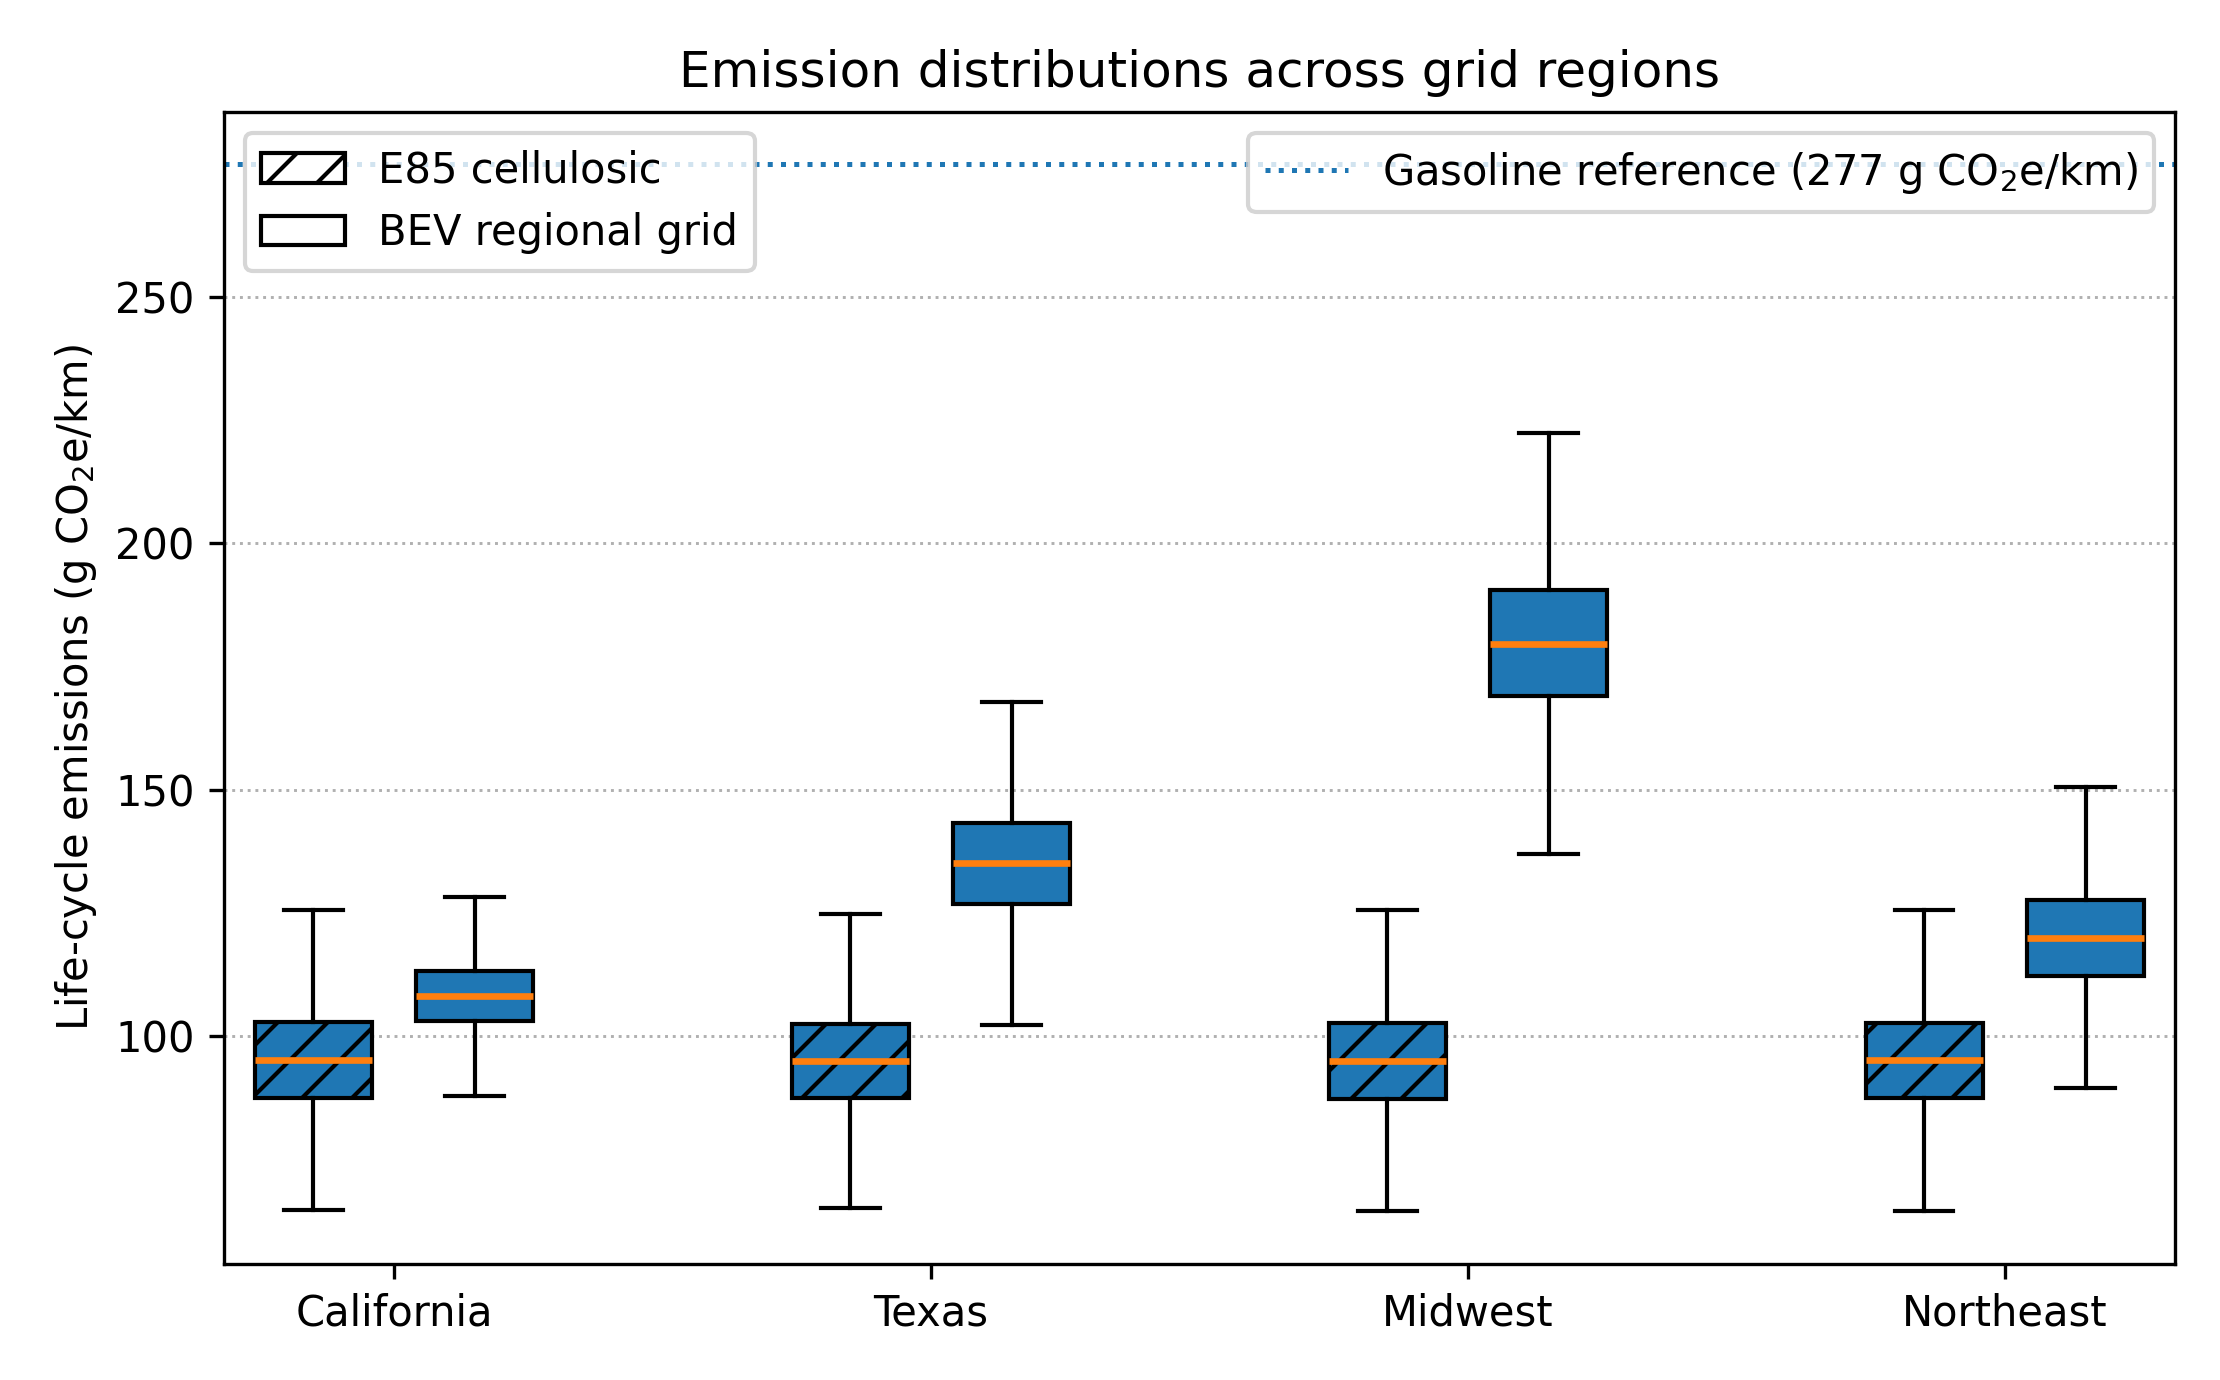
\includegraphics[width=0.90\textwidth]{figures/Figure_1_emission_distributions.png}
	\caption{Emission distributions for cellulosic E85 and BEV operation across grid-zone sensitivity cases. Boxes show Monte Carlo scenario distributions using the parameter values in Table~\ref{tab:parameters}. The dotted reference line indicates gasoline at 277~\gcoeqkm{}. The implemented proof-of-method run is limited to CAISO/CAISO\_NORTH; ERCOT, MISO--MROW, and ISO--NE require equivalent marginal-emissions data before being treated as empirical dispatch results.}
	\label{fig:emission_distributions}
\end{figure}

%\FloatBarrier


\subsection{PHEV emission reductions: CAISO run and extension sensitivity cases}
\label{subsec:phev_reductions}

Table~\ref{tab:regional_reductions} separates the implemented CAISO result from prospective extension cases. In the CAISO case, the populated CSV audit reports that AES reduces PHEV emissions from 181.76 to 123.38~\gcoeqkm{}, a 32.12\% reduction relative to the specified static baseline, with all 168 AES-selected events assigned to cellulosic E85. The ERCOT, MISO--MROW, and ISO--NE rows are not completed empirical dispatch results and should not be cited as regional reductions. They are retained only as hypothetical sensitivity outputs showing how the model would behave under declared extension-zone average factors and scenario inputs.

\begin{table}[htbp]
	\centering
	\begin{threeparttable}
		\caption{PHEV emission changes for AES relative to the static baseline, separated by evidence status.}
		\label{tab:regional_reductions}
		\scriptsize
		\begin{tabular}{lcccl}
			\toprule
			Grid zone & Static baseline & AES optimized & Mean change & Evidence status \\
			& (\gcoeqkm{}) & (\gcoeqkm{}) & (\%) & \\
			\midrule
			CAISO & 181.76 & 123.38 & 32.12 & Implemented CAISO/CAISO\_NORTH proof-of-method run; 168/168 AES selections were cellulosic E85 \\
			ERCOT & 165 & 119 & 28 & Hypothetical extension sensitivity; not empirical \\
			MISO--MROW & 180 & 153 & 15 & Hypothetical extension sensitivity; not empirical \\
			ISO--NE & 155 & 110 & 29 & Hypothetical extension sensitivity; not empirical \\
			\bottomrule
		\end{tabular}
		\begin{tablenotes}
			\footnotesize
			\item Static baseline is defined in Section~\ref{subsec:static_baseline}. Sensitivity values are useful for model exploration but should not be cited as completed regional empirical results until equivalent marginal-emissions, price, and service-event data are supplied.
		\end{tablenotes}
	\end{threeparttable}
\end{table}


\subsection{BEV-only, PHEV, and E85-only comparison}
\label{subsec:pathway_comparison}

Table~\ref{tab:pathway_comparison} is retained as a pathway-comparison scaffold, but the populated CSV audit supplies only the implemented CAISO PHEV proof-of-method values. The uploaded files do not include a separate BEV-only optimized dispatch output; therefore the CAISO BEV-only entry is not populated from the present audit. The PHEV AES and E85-only CAISO entries coincide because the AES dynamic trace selected cellulosic E85 in all 168 events.

\begin{table}[htbp]
	\centering
	\begin{threeparttable}
		\caption{Comparative performance of BEV-only, PHEV with AES, and E85-only operation.}
		\label{tab:pathway_comparison}
		\scriptsize
		\begin{tabular}{lcccl}
			\toprule
			Grid zone & BEV-only optimized & PHEV with AES & E85-only cellulosic & Evidence status \\
			& (\gcoeqkm{}, mean $\pm$ interval) & (\gcoeqkm{}, mean $\pm$ interval) & (\gcoeqkm{}, mean $\pm$ interval) & \\
			\midrule
			CAISO & Not supplied by current audit CSVs & 123.38 & 123.38 & Implemented PHEV proof-of-method; BEV-only requires separate output \\
			ERCOT & $110\pm20$ & $119\pm22$ & $95\pm22$ & Hypothetical extension sensitivity \\
			MISO--MROW & $168\pm29$ & $153\pm24$ & $95\pm22$ & Hypothetical extension sensitivity \\
			ISO--NE & $98\pm18$ & $110\pm20$ & $95\pm22$ & Hypothetical extension sensitivity \\
			\bottomrule
		\end{tabular}
		\begin{tablenotes}
			\footnotesize
			\item Intervals denote propagated scenario uncertainty half-widths, not field-sampling confidence intervals. Extension-zone rows are hypothetical sensitivity outputs and are not completed empirical dispatch runs.
		\end{tablenotes}
	\end{threeparttable}
\end{table}


\subsection{CAISO BEV--cellulosic E85 practical-equivalence result}
\label{subsec:equivalence}

The populated \texttt{equivalence\_tests.csv} output does not support retaining the previous BEV--cellulosic E85 equivalence statement. For the supplied \texttt{PHEV\_FFV\_CAISO} pathway comparison, the mean difference for \texttt{E85\_cellulosic} minus \texttt{electric\_annual\_average} is 28.48~\gcoeqkm{} with a 90\% interval of 28.23--28.73~\gcoeqkm{}, and the test reports \texttt{equivalent=False} for the $\pm10$~\gcoeqkm{} margin. Thus, the current archive supports only a narrower statement: annual-average electric operation is lower than the cellulosic E85 pathway under this PHEV pathway boundary, whereas the AES dynamic dispatch selected E85 in all events because the time-indexed marginal grid intensity during the audited week made electric operation less favorable in the carbon-priority objective. A separate BEV-only optimized output is required before making a BEV--E85 equivalence claim.



\subsection{Battery-production amortization sensitivity}
\label{subsec:battery_sensitivity}

Battery-production terms materially affect cross-technology comparisons. Using the declared battery-production intensity range in Table~\ref{tab:parameters} and a 240,000~km lifetime, a 75~kWh BEV battery contributes 15.6--31.3~\gcoeqkm{} (central value 23.4~\gcoeqkm{} at 75~kg~CO$_2$e/kWh), whereas a 14~kWh PHEV battery contributes 2.9--5.8~\gcoeqkm{} (central value 4.4~\gcoeqkm{}). Table~\ref{tab:battery_sensitivity} shows the arithmetic sensitivity implied by these declared parameters.

\begin{table}[htbp]
\centering
\begin{threeparttable}
\caption{Battery-production amortization sensitivity for declared battery capacities and lifetime.}
\label{tab:battery_sensitivity}
\scriptsize
\begin{tabular}{lccc}
\toprule
Vehicle battery case & 50~kg~CO$_2$e/kWh & 75~kg~CO$_2$e/kWh & 100~kg~CO$_2$e/kWh \\
& (\gcoeqkm{}) & (\gcoeqkm{}) & (\gcoeqkm{}) \\
\midrule
BEV, 75~kWh pack & 15.6 & 23.4 & 31.3 \\
PHEV, 14~kWh pack & 2.9 & 4.4 & 5.8 \\
Incremental BEV minus PHEV battery term & 12.7 & 19.1 & 25.4 \\
\bottomrule
\end{tabular}
\begin{tablenotes}
\footnotesize
\item Values equal battery capacity multiplied by production intensity and divided by 240,000~km. They are not new empirical measurements; they expose the sensitivity already implied by the declared scenario parameters.
\end{tablenotes}
\end{threeparttable}
\end{table}

Because the populated CSV archive does not include a separate BEV-only optimized result, the previous numerical BEV--cellulosic E85 equivalence statement is not retained as an audited finding. Battery-production amortization remains important for any future BEV--PHEV--E85 comparison: adding the central incremental BEV-minus-PHEV battery term of 19.1~\gcoeqkm{} would materially change pathway rankings relative to a smaller-battery PHEV pathway comparison. Consequently, practical-equivalence statements are boundary-dependent and should be reported only when the corresponding BEV, PHEV, and liquid-fuel outputs are archived.

% AUTHOR ACTION REQUIRED: ensure the figure-generation archive records the exact 24-hour date plotted in Figure 2.
\subsection{Example daily dispatch profile}
\label{subsec:dispatch_profile}

Figure~\ref{fig:dispatch_profile} should be interpreted as a dispatch-profile diagnostic generated from the archived run inputs. In the populated CSV audit, however, the carbon-priority AES trace selects cellulosic E85 in all 168 service events and selects no electric charging events. The attached data therefore do not demonstrate within-week electric/E85 switching for this specific run; rather, they show that marginal grid carbon intensity remained high enough that cellulosic E85 was preferred whenever available and compatible.

\begin{figure}[htbp]
	\centering
	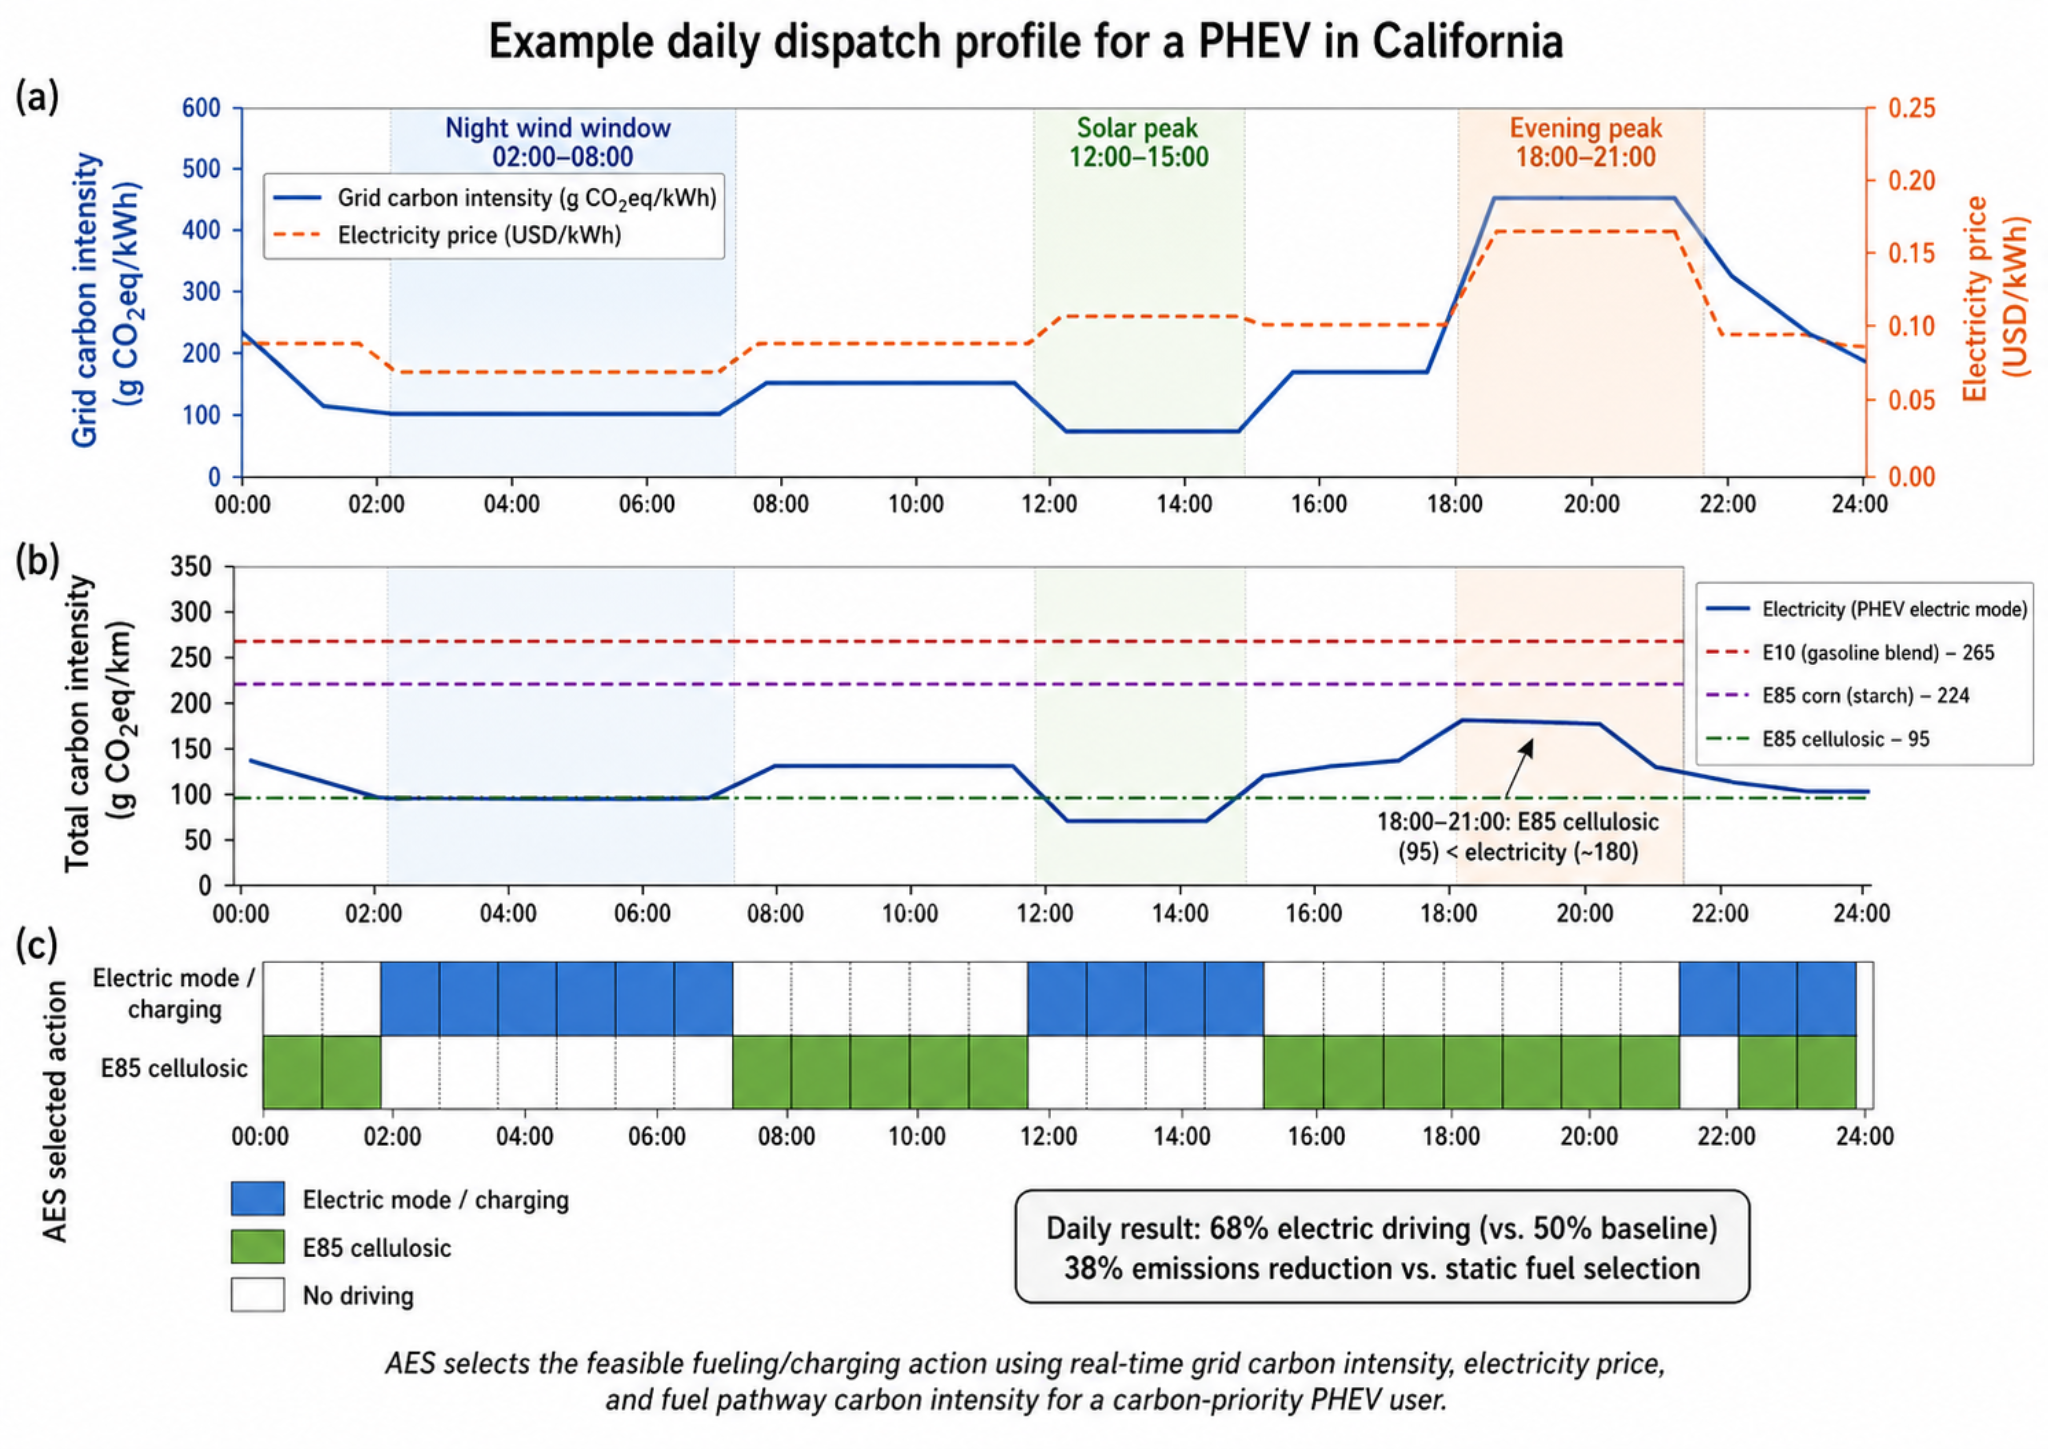
\includegraphics[width=0.92\textwidth]{figures/Figure_2_dispatch_timeseries.png}
	\caption{Example CAISO PHEV dispatch profile for one 24-hour subset of the 1--8 January 2026 proof-of-method interval, generated from the same vehicle parameters listed in Table~\ref{tab:phev_scenario} and the same MOER and price streams used in the CAISO run. Panel (a) reports hourly grid carbon intensity and electricity price; panel (b) compares total pathway carbon intensity for electricity, E10, E85 corn, and E85 cellulosic operation; panel (c) reports the AES-selected action. In panel (c), blue denotes electric mode/charging, green denotes E85 cellulosic operation, and white denotes no driving. The exact date, timestamps, selected actions, and marginal-emissions values must be recoverable from the archived figure-generation input file.}
	\label{fig:dispatch_profile}
\end{figure}

%\FloatBarrier


\section{Discussion}
\label{sec:discussion}

\subsection{Operational carbon information transforms station-level decisions}
\label{subsec:discuss_operational}

Conventional LCA identifies promising technology pathways but cannot resolve the temporal windows during which electricity is substantially cleaner or dirtier than the annual average. The AES formulation bridges this gap by coupling pathway-level carbon-intensity factors with time-resolved marginal grid data and real-time vehicle constraints, enabling a station to generate transaction-level energy recommendations. The populated CAISO proof-of-method supports the narrower proposition that operational carbon information can alter transaction-level fuel choice relative to a static rule: the static baseline contains 85 electric and 83 E10 events, whereas the AES carbon-priority run selects cellulosic E85 in all 168 events. It does not, in this audited run, demonstrate electric/E85 temporal switching; that behavior remains a capability of the formulation to be tested in lower-MOER intervals, alternative fuel availability cases, or seasonal replications.


\subsection{Regional equivalence is conditional and margin-dependent}
\label{subsec:discuss_equivalence}

The populated equivalence-test output should be interpreted more narrowly than the earlier draft. It compares annual-average electric, E10, and cellulosic E85 pathway factors for the PHEV scenario, not a complete BEV-only optimized dispatch case. In that supplied file, \texttt{E85\_cellulosic} exceeds \texttt{electric\_annual\_average} by 28.48~\gcoeqkm{} and is not equivalent at the $\pm10$~\gcoeqkm{} margin. At the same time, the event-level AES dispatch selected E85 for all audited events because the marginal grid intensity during the selected winter week was high. This contrast reinforces the main methodological point: annual-average pathway comparisons and marginal-emissions dispatch decisions answer different questions. The extension cases illustrate conditionality only as hypothetical sensitivities; they are not evidence that the same reduction would occur in MISO--MROW, ERCOT, or ISO--NE without real marginal-emission and price data.


\subsection{Temporal optimization benefits are region-specific}
\label{subsec:discuss_temporal}

The reported 32.12\% emission reduction for the CAISO proof-of-method reflects the specific characteristics of one winter week and the declared service-event stream. It should not be interpreted as annual CAISO performance, as representative of summer or shoulder-season renewable patterns, or as a transferable regional reduction. The magnitude of temporal optimization benefits will differ in other regions depending on marginal-emission profiles, grid composition, price structures, and the flexibility of vehicle operators to shift charging times. This pattern is consistent with the broader smart-charging literature~\cite{GraffZivin2014,Holland2016} and motivates seasonal replications before policy generalization.


\subsection{PHEV operational flexibility and its limits}
\label{subsec:discuss_phev}

PHEVs are well suited to AES control because they expand the feasible action set beyond what is available to BEV-only or liquid-fuel-only vehicles. However, the results do not support characterizing PHEVs as universally superior. Their advantage is conditional resilience: the ability to use electricity when the grid is clean, switch to certified low-carbon liquid fuel when marginal emissions are elevated, and retain liquid-fuel range where charging infrastructure is limited. This flexibility depends on actual driver willingness to charge, charger access, dwell time, battery state, and verified fuel availability. As grids decarbonize and charging infrastructure matures, or if low-carbon liquid fuels are unavailable, the marginal value of PHEV flexibility may diminish --- a trajectory that the AES framework can track through updated marginal-emission and availability inputs.


\subsection{Policy implications}
\label{subsec:discuss_policy}

The modeling results support technology-neutral, performance-based policies that reward verified carbon-intensity reductions rather than prescribing a single vehicle technology for all regions. Low-carbon fuel standards, clean electricity standards, smart-charging mandates, open marginal-emission data requirements, and station-level carbon reporting could all facilitate AES deployment. However, the policy interpretation is derived from regional and temporal variability in the model, not from a randomized policy trial. Public incentives should therefore be conditioned on measured carbon performance, infrastructure utilization, equitable user access, cybersecurity assurance, and verified supply-chain sustainability.


\subsection{Limitations}
\label{subsec:limitations}

Several limitations warrant acknowledgment. First, the executable implementation covers only one CAISO/CAISO\_NORTH winter week (1--8 January 2026), which includes holiday-period operating conditions and should not be interpreted as seasonally or annually representative. A more robust assessment should incorporate stratified weeks or full-year runs covering seasonal variation, weekday/weekend effects, and high- versus low-renewable intervals. Second, the reported implementation uses hourly service events; no separate 5-minute station-control simulation is claimed. Third, user behavior is uncertain --- drivers may ignore recommendations, prioritize travel time, refuse higher-cost lower-carbon options, or arrive with unexpected state-of-charge. The model represents user classes through fixed weights, but real behavior should be estimated from field trials. Fourth, infrastructure constraints are simplified: charger queues, feeder capacity, dispenser availability, E85 distribution, and station inventory can all constrain feasible dispatch. Queue penalties are inactive in the reported run and should be activated only when station-traffic data are available. Fifth, the cellulosic E85 pathway is a scenario option, not a claim of broad retail availability; deployment studies need supply constraints, certification, and station inventory data. Sixth, carbon-priority operation is the headline scenario, while a real station must consider cost, queueing, customer acceptance, and contractual constraints. Seventh, cybersecurity risks are material --- AES depends on external data feeds, vehicle-to-infrastructure communication, and station controllers. Data spoofing or compromised carbon-intensity signals could produce incorrect recommendations; future deployments should include signed data streams, local fallback profiles, and anomaly detection. Eighth, infrastructure LCA and consequential market effects are excluded; large-scale AES deployment could affect electricity demand, ethanol markets, land use, and grid congestion, requiring consequential LCA and integrated energy-system modeling.


\section{Conclusions}
\label{sec:conclusions}

This study presents an AES framework for life-cycle-aware, time-resolved dispatch of electric charging and low-carbon liquid fuels at multi-fuel transport-energy stations. The main conclusions are:

\begin{enumerate}
	\item Static LCA is necessary but insufficient for station-level operational decisions because grid carbon intensity, prices, and feasible vehicle actions vary over time.
	
	\item In the CAISO/CAISO\_NORTH proof-of-method case with 168 hourly service events over one winter week, 1--8 January 2026 Pacific time, AES-controlled PHEV operation reduces the reported scenario mean from 181.76 to 123.38~\gcoeqkm{} relative to the specified static baseline. This is not an annual CAISO result, not a fleet-adoption forecast, and not transferable without seasonal replication.
	
	\item ERCOT, MISO--MROW, and ISO--NE values are hypothetical extension sensitivity outputs, not completed empirical regional dispatch results; they should not be cited as measured regional reductions.
	
	\item The populated \texttt{equivalence\_tests.csv} file does not support retaining the earlier BEV--cellulosic E85 equivalence claim as an audited result. It reports a PHEV-pathway comparison in which \texttt{E85\_cellulosic} exceeds \texttt{electric\_annual\_average} by 28.48~\gcoeqkm{} and is not equivalent at the $\pm10$~\gcoeqkm{} margin. A separate BEV-only optimized output is required before making a BEV--E85 equivalence claim.
	
	\item PHEVs should not be described as universally superior; their AES value is conditional operational flexibility across changing grid, price, infrastructure, driver-behavior, and certified fuel-supply conditions.
\end{enumerate}

The policy conclusion is separate from the statistical results: AES can support performance-based, regionally flexible decarbonization policy only if data transparency, event-level dispatch auditing, infrastructure availability, cost sensitivity, user behavior, cybersecurity, and supply-chain sustainability are addressed.


\section*{Data Availability Statement}

The reproducibility package includes: (i) source code for CAISO OASIS price retrieval, WattTime MOER retrieval, AES input population, validation, dispatch, Monte Carlo uncertainty propagation, sensitivity analysis, and figure generation; (ii) the CAISO/CAISO\_NORTH input tables for the one-week proof-of-method run; (iii) output CSV files used to generate all tables and figures; (iv) event-level dispatch-audit files reporting selected actions, rejected feasible actions, MOER values, prices, SOC reason codes, and action counts; (v) a README with exact commands, package versions, random seeds, and units; (vi) a data dictionary identifying entries as measured, source-derived, or scenario inputs; and (vii) a machine-readable run manifest with retrieval dates, row counts, units, and SHA-256 checksums. The reproducibility package, including all data and source code, has been archived and publicly released through GitHub at \url{https://github.com/marcobernardes/AES}. ERCOT, MISO--MROW, and ISO--NE extensions require equivalent marginal-emissions access and are not represented as completed empirical runs in the current archive.



\section*{Declaration of generative AI and AI-assisted technologies in the manuscript preparation process}

During manuscript preparation, the author used AI-assisted tools for editorial drafting, LaTeX formatting, and consistency checking. The author reviewed and edited the content and takes full responsibility for the final manuscript.


\section*{CRediT authorship contribution statement}

\textbf{Marco Aur\'elio dos Santos Bernardes:} Conceptualization, Methodology, Software, Formal analysis, Writing -- original draft, Writing -- review \& editing.


\section*{Declaration of competing interest}

The author declares no known competing financial interests or personal relationships that could have appeared to influence the work reported in this paper.




% Add acknowledgements here if applicable.
% If no funding: This research did not receive any specific grant from funding agencies in the public, commercial, or not-for-profit sectors.

\section*{Acknowledgements}
This research did not receive any specific grant from funding agencies 
in the public, commercial, or not-for-profit sectors.

\section*{Nomenclature }


\begin{table}[htbp]
	\centering
	%\caption{Symbols and Descriptions}
	\label{tab:symbols}
	\begin{tabular}{l p{0.65\linewidth}}
		\toprule
		\textbf{Symbol} & \textbf{Description} \\
		\midrule
		$C_{i,t}$      & Carbon intensity per km for action $i$ at time $t$ \\
		$K_{i,t}$      & Cost per km for action $i$ at time $t$ \\
		$w_C, w_{\$}$  & Carbon and cost preference weights \\
		$\mathcal{F}_{v,t}$ & Feasible action set for vehicle $v$ at event $t$ \\
		$M_t$          & Marginal operating emissions rate at time $t$ \\
		$E_{v,i}$      & Vehicle energy use per km \\
		$\Delta$       & Practical-equivalence margin \\
		$\epsilon$     & Numerical stability constant \\
		$\lambda_T, \lambda_Q$ & Time and queue penalty coefficients \\
		SOC            & State of charge \\
		MOER           & Marginal operating emissions rate \\
		LMP            & Locational marginal price \\
		CI             & Carbon intensity \\
		CV             & Coefficient of variation \\
		\bottomrule
	\end{tabular}
\end{table}












%%%%%%%%%%%%%%%%%%%%%%%%%%%%%%%%%%%%%%%%%%
%\isPreprints{}{% This command is only used for ``preprints''.
%%%%%%%%%%%%%%%%%%%%%%%%%%%%%%%%%%%%%%%%%%
%
\begin{adjustwidth}{-\extralength}{0cm}
%\printendnotes[custom]

\reftitle{References}

\begin{thebibliography}{999}
\bibitem[Argonne National Laboratory(2023)]{Argonne2023}
Argonne National Laboratory, GREET 2023 Model, Argonne, IL, 2023.
\bibitem[Bernardes(2009)]{Bernardes2009}
M.A.S. Bernardes, Life cycle assessment modeling for bifuel vehicles in Brazil, 2009.
\bibitem[California ISO(2017)]{CAISOOASISAPI}
California ISO, OASIS interface specification, version 4.3.5, 2017.
\bibitem[California ISO(2025)]{CAISOOASISFAQ}
California ISO, Open Access Same-time Information System (OASIS) frequently asked questions, 2025.
\bibitem[Duoba et al.(2026)]{Duoba2026}
M. Duoba, J.P. González, Modeling real-world charging behavior to update SAE J2841 PHEV utility factors, World Electric Vehicle Journal 17(5) (2026) 242. doi:10.3390/wevj17050242.
\bibitem[Earles et al.(2011)]{Earles2011}
J.M. Earles, A. Halog, Consequential life cycle assessment: A review, International Journal of Life Cycle Assessment 16 (2011) 445--453. doi:10.1007/s11367-011-0275-9.
\bibitem[Elgowainy et al.(2018)]{Elgowainy2018}
A. Elgowainy, J. Han, J. Ward, F. Joseck, D. Gohlke, A. Lindauer, T. Ramsden, M. Biddy, M. Alexander, S. Barnhart, I. Sutherland, L. Verduzco, T.J. Wallington, Cradle-to-grave lifecycle analysis of U.S. light-duty vehicle-fuel pathways: A greenhouse gas emissions and economic assessment of current (2015) and future (2025-2030) technologies, Argonne National Laboratory, ANL/ESD-16/7 Rev. 1, Lemont, IL, 2018. \url{https://greet.es.anl.gov/}.
\bibitem[Ellingsen et al.(2014)]{Ellingsen2014}
L.A.W. Ellingsen, G. Majeau-Bettez, B. Singh, A.K. Srivastava, L.O. Valøen, A.H. Strømman, Life cycle assessment of a lithium-ion battery vehicle pack, Journal of Industrial Ecology 18(1) (2014) 113--124. doi:10.1111/jiec.12072.
\bibitem[U.S. Environmental Protection Agency(2025)]{EPAeGRID2023}
U.S. Environmental Protection Agency, eGRID2023 summary tables and Emissions \& Generation Resource Integrated Database, 2025.
\bibitem[Fraunhofer ISI(2025)]{Fraunhofer2025}
Fraunhofer ISI, Regulatory adjustments for plug-in hybrid vehicles in Europe, Fraunhofer Institute for Systems and Innovation Research, Karlsruhe, Germany, 2025. \url{https://www.ifeu.de/fileadmin/uploads/Publikationen/Mobilit\%C3\%A4t/Plugin-Hybrid_Dateien/Analyse_PHEV_2025_EN_final.pdf}.
\bibitem[Geisler et al.(2005)]{Geisler2005}
G. Geisler, S. Hellweg, K. Hungerbühler, Uncertainty analysis in life cycle assessment using generic uncertainty factors, International Journal of Life Cycle Assessment 10(4) (2005) 248--257. doi:10.1065/lca2004.09.177.
\bibitem[Graff Zivin et al.(2014)]{GraffZivin2014}
J.S. Graff Zivin, M.J. Kotchen, E.T. Mansur, Spatial and temporal heterogeneity of marginal emissions: Implications for electric cars and other electricity-shifting policies, Journal of Economic Behavior \& Organization 107 (2014) 248--268. doi:10.1016/j.jebo.2014.03.010.
\bibitem[Hawkes(2014)]{Hawkes2014}
A.D. Hawkes, Long-run marginal CO$_2$ emissions factors in national electricity systems, Applied Energy 125 (2014) 197--205. doi:10.1016/j.apenergy.2014.03.060.
\bibitem[Holland et al.(2016)]{Holland2016}
S.P. Holland, E.T. Mansur, N.Z. Muller, A.J. Yates, Are there environmental benefits from driving electric vehicles? The importance of local factors, American Economic Review 106(12) (2016) 3700--3729. doi:10.1257/aer.20150897.
\bibitem[ISO(2006a)]{ISO2006a}
ISO, ISO 14040: Environmental management -- Life cycle assessment -- Principles and framework, International Organization for Standardization, Geneva, 2006.
\bibitem[ISO(2006b)]{ISO2006b}
ISO, ISO 14044: Environmental management -- Life cycle assessment -- Requirements and guidelines, International Organization for Standardization, Geneva, 2006.
\bibitem[Liska et al.(2009)]{Liska2009}
A.J. Liska, H.S. Yang, V.R. Bremer, T.J. Klopfenstein, D.T. Walters, G.E. Erickson, K.G. Cassman, Improvements in life cycle energy efficiency and greenhouse gas emissions of corn-ethanol, Journal of Industrial Ecology 13 (2009) 58--74.
\bibitem[Menten et al.(2013)]{Menten2013}
F. Menten, B. Chèze, L. Patouillard, F. Bouvart, A review of LCA greenhouse gas emissions results for advanced biofuels: The use of meta-regression analysis, Renewable and Sustainable Energy Reviews 26 (2013) 108--134. doi:10.1016/j.rser.2013.04.021.
\bibitem[Messagie et al.(2014)]{Messagie2014}
M. Messagie, F.-S. Boureima, T. Coosemans, C. Macharis, J. Van Mierlo, A range-based vehicle life cycle assessment incorporating variability in the environmental assessment of different vehicle technologies and fuels, Energies 7(3) (2014) 1467--1482. doi:10.3390/en7031467.
\bibitem[Miller et al.(2021)]{Miller2021}
I. Miller, E. Gençer, Hourly accounting of carbon emissions from electricity consumption, Environmental Science \& Technology 55(16) (2021) 11091--11099. doi:10.1021/acs.est.1c00864.
\bibitem[Pfenninger et al.(2017)]{Pfenninger2017}
S. Pfenninger, J. DeCarolis, L. Hirth, S. Quoilin, I. Staffell, The importance of open data and software: Is energy research lagging behind?, Energy Policy 101 (2017) 211--215. doi:10.1016/j.enpol.2016.11.046.
\bibitem[Plötz et al.(2020)]{Plotz2020b}
P. Plötz, C. Moll, Y. Li, G. Bieker, P. Mock, Real-world usage of plug-in hybrid electric vehicles in China, Europe, and North America, Transportation Research Part D: Transport and Environment 84 (2020) 102365. doi:10.1016/j.trd.2020.102365.
\bibitem[Sandve et al.(2013)]{Sandve2013}
G.K. Sandve, A. Nekrutenko, J. Taylor, E. Hovig, Ten simple rules for reproducible computational research, PLOS Computational Biology 9(10) (2013) e1003285. doi:10.1371/journal.pcbi.1003285.
\bibitem[Scown et al.(2012)]{Scown2012}
C.D. Scown, W.W. Nazaroff, U. Mishra, B. Strogen, A.B. Lobscheid, E. Masanet, N.J. Santero, A. Horvath, T.E. McKone, Lifecycle greenhouse gas implications of US national scenarios for cellulosic ethanol production, Environmental Research Letters 7(1) (2012) 014011. doi:10.1088/1748-9326/7/1/014011.
\bibitem[Vandepaer et al.(2019)]{Vandepaer2019}
L. Vandepaer, K. Treyer, C. Mutel, C. Bauer, B. Amor, The integration of long-term marginal electricity supply mixes in the ecoinvent consequential database version 3.4 and examination of modeling choices, International Journal of Life Cycle Assessment 24 (2019) 1409--1428. doi:10.1007/s11367-018-1571-4.
\bibitem[Wang et al.(2012)]{Wang2012}
M. Wang, J. Han, J.B. Dunn, H. Cai, A. Elgowainy, Well-to-wheels energy use and greenhouse gas emissions of ethanol from corn, sugarcane and cellulosic biomass for US use, Environmental Research Letters 7(4) (2012) 045905. doi:10.1088/1748-9326/7/4/045905.
\bibitem[WattTime(2024)]{WattTime2024}
WattTime, How emissions-optimized EV charging enables cleaner electric vehicles, WattTime, Oakland, CA, 2024. \url{https://watttime.org/wp-content/uploads/2024/01/WattTime-EVAnalysis-FullReport-vFinal.pdf}.
\bibitem[WattTime(2026a)]{WattTimeAPI}
WattTime, WattTime data API documentation, 2026.
\bibitem[WattTime(2024)]{WattTimeMOER}
WattTime, Marginal operating emissions rate (MOER) data signal and API documentation, 2024.
\bibitem[Wernet et al.(2016)]{Wernet2016}
G. Wernet, C. Bauer, B. Steubing, J. Reinhard, E. Moreno-Ruiz, B. Weidema, The ecoinvent database version 3 (part I): Overview and methodology, International Journal of Life Cycle Assessment 21 (2016) 1218--1230.
\end{thebibliography}

\PublishersNote{}
\end{adjustwidth}
\end{document}
